\documentclass[manuscript]{acmart}

\usepackage{mathtools}
\usepackage{enumitem}
\usepackage{url}
\usepackage{tikz}
\urlstyle{tt}
\DeclareUrlCommand\path{\urlstyle{tt}}
\makeatletter
\g@addto@macro\UrlBreaks{\do\_\do\-}
\makeatother
\usetikzlibrary{arrows.meta,positioning,decorations.pathreplacing,automata,calc}
% Unified monochrome figure style for the paper.
% All automata and timing diagrams use white states, black borders and black arrows.
\tikzset{
  fmbracebottom/.style={
    decorate,
    decoration={brace,mirror,amplitude=4pt}
  },
  fmstate/.style={
    circle, draw=black, fill=white, line width=0.6pt,
    minimum size=9mm, inner sep=1pt, font=\small
  },
  fmstatewide/.style={
    rounded rectangle, draw=black, fill=white, line width=0.6pt,
    minimum height=8mm, inner xsep=3pt, inner ysep=1.5pt, font=\small
  },
  fmaccept/.style={fmstate,double,double distance=1.2pt},
  fmerror/.style={fmstate,double,double distance=1.2pt,fill=white},
  fmedge/.style={->,>=Stealth,line width=0.6pt},
  fmlabel/.style={font=\scriptsize,align=center,fill=white,inner sep=1.2pt},
  fminvariant/.style={font=\scriptsize,align=center},
  fmnote/.style={font=\scriptsize,align=center},
  fmtimeline/.style={->,>=Stealth,line width=0.6pt},
  fmevent/.style={circle,draw=black,fill=white,line width=0.6pt,minimum size=4.5mm,inner sep=0.5pt},
  fmreference/.style={fmevent,double,double distance=0.8pt},
  fmguide/.style={densely dashed,line width=0.45pt},
  fmbrace/.style={decorate,decoration={brace,amplitude=4pt},line width=0.5pt}
}

\AtBeginDocument{\theoremstyle{acmdefinition}\newtheorem{assumption}[theorem]{Assumption}}

\newcommand{\Nat}{\mathbb{N}}
\newcommand{\Real}{\mathbb{R}}
\newcommand{\satM}{\models_{\mathrm{MTL}}}
\newcommand{\satL}{\models_{\mathrm{LTL}}}
\newcommand{\Until}{\mathbin{\mathsf{U}}}
\newcommand{\Release}{\mathbin{\mathsf{R}}}
\newcommand{\hUntil}{\mathbin{\widehat{\mathsf{U}}}}
\newcommand{\hRelease}{\mathbin{\widehat{\mathsf{R}}}}
\newcommand{\Next}{\mathsf{X}}
\newcommand{\Always}{\mathsf{G}}
\newcommand{\Eventually}{\mathsf{F}}
\newcommand{\WeakUntil}{\mathbin{\mathsf{W}}}
\providecommand{\Reset}{}\renewcommand{\Reset}{\mathsf{rst}}
\newcommand{\Unch}{\mathsf{unch}}
\newcommand{\T}{\mathcal{T}}
\newcommand{\Node}{\mathsf{node}}
\newcommand{\CVal}{\mathsf{val}}
\newcommand{\CReset}{\mathsf{reset}}
\newcommand{\elapsed}{\mathsf{elap}}
\newcommand{\ewbase}{\mathsf{ew\_base}}
\newcommand{\Clock}{\mathit{Clock}}
\newcommand{\runinhead}[1]{\par\noindent\textbf{#1}\enspace}
\newcommand{\Rocqid}[1]{\url{#1}}

\acmJournal{TOCL}

\begin{document}

\title{A Mechanically Checked Translation of MTL$_{0,\infty}$ into Timed B\"uchi Automata via Clocked LTL}

\author{Elie Fares}
\email{efares@hct.ac.ae}
\affiliation{\institution{Higher Colleges of Technology}\city{Sharjah}\country{United Arab Emirates}}
\author{Jean-Paul Bodeveix}
\email{bodeveix@irit.fr}
\affiliation{\institution{IRIT, Universit\'e de Toulouse}\city{Toulouse}\country{France}}
\author{Hussain Al-Aqrabi}
\email{halaqrabi@hct.ac.ae}
\affiliation{\institution{Higher Colleges of Technology}\city{Sharjah}\country{United Arab Emirates}}
\author{Azar Salami}
\email{asalami@hct.ac.ae}
\affiliation{\institution{Higher Colleges of Technology}\city{Sharjah}\country{United Arab Emirates}}

\begin{abstract}
Timed model checkers operate on timed B\"uchi automata (TBAs), so the translation
of Metric Temporal Logic (MTL$_{0,\infty}$) into a TBA is the semantic link
between a requirement and every analysis of it. We present a Rocq-checked proof
that this translation, factored through clocked Linear Temporal Logic (LTL),
preserves the timed-word language under a pointwise semantics. Earlier constructions (Bulychev et~al.,
Li et~al.) extend the tableau LTL-to-B\"uchi translation with clocks directly;
their paper proofs treat some cases as similar to others and omit them. Here the
formula is instead encoded into an untimed clocked-LTL formula that a standard
LTL-to-B\"uchi backend processes, and relaxation and reset completion restore
the timed meaning. The encoding is proved sound and complete for all eight
primitive timed cases, with a canonical reset trace for shared clocks. The
resulting TBA is correct for every backend that meets an explicit
language-equivalence contract, and we prove the contract in Rocq for a
verified LTL-to-B\"uchi construction, so the main theorem holds with no assumption on the
backend beyond the standard Rocq axioms. A second main result isolates the
relaxation and reset-completion stage: it is proved for positive clocked-LTL
formulas over an abstract clock type whose clocks satisfy an explicit polarity
condition, with the MTL translation as an instance; two counterexamples show that
the condition cannot simply be dropped, and the theorem covers one fixed reset
rule and event-guarded automata, not arbitrary timed logics. We are not aware of
an earlier presentation of the translation in this factored form, or of a
published machine-checked development of a pointwise MTL$_{0,\infty}$-to-TBA
construction. The verified backend is a proof witness and is not
the one used by the extracted tool \texttt{mtl2tba}, which calls Spot; the tool
and its parser, graph import and extraction lie outside the checked boundary.
\end{abstract}

\begin{CCSXML}
<ccs2012>
<concept><concept_id>10003752.10003790</concept_id><concept_desc>Theory of computation~Logic</concept_desc><concept_significance>500</concept_significance></concept>
<concept><concept_id>10003752.10003766.10003773.10003775</concept_id><concept_desc>Theory of computation~Timed and hybrid models</concept_desc><concept_significance>500</concept_significance></concept>
<concept><concept_id>10003752.10003790.10002990</concept_id><concept_desc>Theory of computation~Logic and verification</concept_desc><concept_significance>300</concept_significance></concept>
</ccs2012>
\end{CCSXML}
\ccsdesc[500]{Theory of computation~Logic}
\ccsdesc[500]{Theory of computation~Timed and hybrid models}
\ccsdesc[300]{Theory of computation~Logic and verification}

\keywords{Metric temporal logic, timed B\"uchi automata, Rocq, mechanized proof, clocked LTL, translation correctness}

\maketitle

\section{Introduction}
\label{sec:introduction}
Metric Temporal Logic (MTL) specifies real-time requirements, and timed
B\"uchi automata (TBAs) are the model on which timed model checkers operate.
The translation of an MTL formula into a TBA is therefore the semantic link
between a requirement and every automata-based analysis of it; if it is wrong,
no verdict built on it may say anything about the requirement. The translation is
also delicate. Timed subformulas share clocks, and the obligations of
overlapping activations must be served by a single clock. A bounded-response
requirement, for example, is
\begin{equation*}
\Box(\mathit{req}\Rightarrow\Diamond_{\le d}\mathit{ack}).
\end{equation*}
With $d=5$, requests at times 0 and 4 and an acknowledgment at time 6 violate
the first request's deadline, yet a naive single clock reset at every request
reads only 2 at the acknowledgment. The reset semantics therefore needs a
correctness argument.

\runinhead{Main result.} We prove in Rocq that the pointwise
MTL$_{0,\infty}$-to-TBA translation, factored
through clocked LTL, preserves the timed-word language. The semantics is the
pointwise semantics defined in Section~\ref{sec:logic}, with one action per
position. For every well-formed
formula $f$ and every backend automaton that meets the backend contract
(Assumption~\ref{ass:backend}) for the clocked-LTL encoding $\T(f)$, the timed
automaton obtained by relaxation and reset completion accepts exactly the timed
words that satisfy $f$ (Theorem~\ref{thm:mtl-to-tba-correct},
\Rocqid{MTL_to_TBA_correct_with}). We also prove the contract in Rocq for a
simple LTL-to-B\"uchi construction of the Miyano--Hayashi type
(Section~\ref{subsec:verified-backend}), so that the theorem holds for the
translation with that backend with no assumption beyond the standard Rocq
axioms (Theorem~\ref{thm:verified}, \Rocqid{MTL_to_TBA_correct_verified}). The
tool calls Spot instead, for efficiency; the precise boundary of what is and is
not checked is given under \emph{Scope of the result} below and in
Section~\ref{subsec:rocq-result-map}.

The construction has predecessors: Bulychev et~al.~\cite{BDLG14} prove exact timed-automaton language results for the safety
and co-safety fragments, with several cases omitted as similar. Li et~al. prove
full-fragment MTL$_{0,\infty}$-to-TBA language equality and language
preservation under their best-choice reset policy, in an appendix of the
version we consulted~\cite{li_spin7}, again omitting cases as similar. Their
work already contains the central timed-subformula clocking and reset
architecture. They build the timed B\"uchi automaton directly, by extending the
classical tableau translation with clocks. We keep that clocking and reset
architecture but reformulate it: the formula is encoded into an untimed formula of clocked Linear Temporal Logic (LTL), a standard LTL-to-B\"uchi backend is applied through an
explicit contract, and relaxation and reset completion restore the timed
meaning. Our contribution is this reformulation and its machine-checked proof.
Table~\ref{tab:prior-construction-comparison} compares these
constructions.

\runinhead{What is new beyond existing correctness results.}
The clock-per-timed-subformula architecture and language equality for
integer bounds are known: proved, with some cases omitted as similar, for the safety and
co-safety fragments~\cite{BDLG14} and for the full fragment~\cite{li_spin7}. We do not present shared
clocks or reset policies as new. In the model of this article we prove, and
machine-check, four results; the first three build on one another, and the
fourth does not depend on MTL. First, a global completeness argument for the
factored encoding: one canonical reset trace serves every syntactic occurrence
and every overlapping activation of a shared clock, for all eight primitive
cases with strict and non-strict bounds
(Theorem~\ref{thm:canonical-all}). Second, a modular correctness theorem: the
timed argument is proved once, for every LTL-to-B\"uchi backend that meets an
explicit language contract, so correctness splits into two independently
specified obligations, encoding equivalence and the backend contract
(Theorem~\ref{thm:mtl-to-tba-correct}). Third, a verified backend that
discharges the contract, which makes the modular theorem unconditional
(Theorem~\ref{thm:verified}). Both the contract-parametric theorem and the
canonical-trace argument are independent of any particular backend or tool: a
future verified backend plugs into the former without repeating the timed proof.
Fourth, the passage from a propositional B\"uchi automaton to a TBA, that is,
relaxation and reset completion, is proved for every positive clocked-LTL
formula over an abstract clock type that meets a syntactic polarity condition,
with the MTL theorem as an instance (Theorem~\ref{thm:general}). This isolates
the part of the proof that does not depend on MTL and makes explicit the
assumptions on which it relies: one fixed reset rule, positive formulas, the
polarity condition, and event-guarded TBAs. Two counterexamples show that the
polarity condition cannot be omitted for this reset rule, and an illustrative
example shows two clock kinds in one non-MTL formula
(Section~\ref{subsec:general}). The theorem is not a verified compiler for
arbitrary timed logics.
The proof also goes beyond the cases the earlier rules cover. Those rules treat
the four non-strict ordinary operators, with strict bounds only in the
semantics; here the hatted operators, strict and non-strict bounds,
nondecreasing timestamps, and arbitrary nonnegative initial
clocks are all covered. Where the earlier paper proofs omit cases as similar, the development gives
a machine-checked proof of language equality for our construction with no case
omitted, in our model and for core formulas: the
reductions for zero bounds described in Section~\ref{sec:logic} are applied
before encoding and are not mechanized. It is therefore not a proof of the
statement of Li et~al. in their own semantics.
\begin{table*}[!t]
\centering
\caption{Representative mathematical results and mechanization evidence for
selected timed-logic-to-automata constructions. The rows have different logics,
semantics, targets, and proof scopes; they are not a performance comparison}
\label{tab:prior-construction-comparison}
\footnotesize\setlength{\tabcolsep}{3pt}
\begin{tabular}{@{}p{0.13\textwidth}p{0.20\textwidth}p{0.36\textwidth}p{0.26\textwidth}@{}}
\toprule
Work & Semantic scope & Existing correctness and construction & Mechanization and implementation evidence\\
\midrule
Bulychev et~al.~\cite{BDLG14} & Pointwise non-Zeno infinite words; integer bounds, all four comparisons in the semantics (the rewriting rules cover only the non-strict ordinary operators), nondecreasing timestamps. & Theorems 1--2 prove exact automaton languages for safety/co-safety; several cases are omitted as similar. The construction extends the classical tableau LTL-to-B\"uchi translation directly, with timed-subformula clocks, obligations, and reset/unchanged markers. & Mathematical proofs and controller-synthesis tooling for the stated fragments.\\
Li et~al.~\cite{li_spin7} & Full MTL$_{0,\infty}$; pointwise non-Zeno words, integer bounds, all four comparisons, nondecreasing timestamps, zero initial clocks. & Proves exact language equality for the timed-B\"uchi construction (closure, extended formulas, degeneralization) and language preservation under best-choice resets, in an appendix; remaining cases are omitted as similar. & CASAAL implements the workflow and deterministic approximations~\cite{casaal_tool}.\\
Xu and Miao~\cite{xu08} & MITL formulas mapped to fair timed automata; exact semantic relation to this paper's pointwise event-word model is not compared. & One tester automaton per subformula, with local clocks measuring elapsed time against the metric interval, composed in parallel; no intermediate untimed LTL stage. & The construction and its implementation in PVS; whether a correctness proof was mechanized is not established here.\\
This article & Well-formed Rocq formulas with real bounds, nondecreasing timestamps, divergent (non-Zeno) timestamps, existentially quantified nonnegative initial clocks (zero initial clocks give the same
language, Corollary~\ref{cor:zero-init}). & Translation factored through clocked LTL and a standard LTL-to-B\"uchi backend. \Rocqid{EncodingCorrect_proved} proves clocked-LTL equivalence for all eight primitive cases; TBA composition holds for any backend meeting the contract, and unconditionally for a verified backend. & Rocq-checked proof, a verified backend, and one proved contract for a manual Spot transcription; a tool with extracted code (Section~\ref{sec:evaluation}).\\
\bottomrule
\end{tabular}
\end{table*}

Mathematical proofs and machine-checked proofs provide different assurance.
A proof assistant requires the syntax, timed-word semantics, clock updates,
invariants, quantifiers, and proof dependencies to be represented in a
kernel-checkable development. Here that formalization must also reconcile
propositions of clocked LTL with genuine clock
valuations. Related proof-assistant
work addresses neighboring problems: Xu and Miao present a Metric Interval
Temporal Logic (MITL)-to-fair-timed-automaton construction and discuss its
implementation in the Prototype Verification System (PVS); Roohi and
Viswanathan mechanize results for MITL decision procedures in PVS; Schimpf et~al. verify an LTL-to-B\"uchi construction in Isabelle's higher-order logic
(HOL); Wang et~al. verify a
Metric Linear Temporal Logic (MLTL)-to-regular-expression transformation in
Isabelle/HOL; and Chattopadhyay and Mamouras mechanize online monitoring for
past-time MTL under discrete-time quantitative semantics
\cite{xu08,roohi_viswanathan_vmcai18,schimpf_tphols09,
wang_mltl_tacas25,chattopadhyay_mamouras_rv20}.

Several interacting proof obligations make the mechanization nontrivial.
Soundness must hold for every clock-consistent reset trace;
completeness must construct one trace that supports every dynamic activation
of a shared, formula-keyed clock. Independent witnesses per activation cannot
establish this single-trace property. The proof maintains residual obligations
for upper- and lower-bound Until and Release, and uses occurrence-indexed
structural induction so recursion through a syntax path retains the clock
identity of an identical primitive formula. In addition, the propositional backend can
assign clock atoms independently of actual clock valuations, so relaxation
and reset completion must preserve the precise implication directions before
the automaton theorem can be composed.

\runinhead{Proof architecture.} The proof has two halves, which
Figure~\ref{fig:correctness-composition} composes for the completeness and
soundness directions. The first proves that the encoding
$\T(f)$ is equivalent to $f$ over clock-consistent extended words:
soundness for arbitrary reset traces, one primitive case at a time
(Section~\ref{subsec:primitive-soundness}), and completeness for one canonical
reset trace (Sections~\ref{subsec:canonical-policy}
and~\ref{subsec:primitive-completeness}), both lifted from primitives to whole
formulas by the occurrence-indexed induction of
Section~\ref{subsec:occurrence-induction}. The second half passes from clocked
LTL to a TBA: the backend contract gives a propositional B\"uchi automaton for
$\T(f)$, and relaxation and reset completion
(Section~\ref{sec:reset-completion}) turn it into a TBA with the same timed
language. Section~\ref{subsec:rocq-result-map} maps each step to its Rocq
theorem and lists the assumptions. Section~\ref{subsec:verified-backend} discharges the
contract in general with a verified backend, and Section~\ref{sec:alarm-example}
gives one small concrete instance of the contract.

The principal contributions are:
\begin{itemize}
  \item a reformulation of the construction that factors the translation
        through an untimed clocked-LTL formula and a standard
        LTL-to-B\"uchi backend, with the backend as an explicit language
        contract, in contrast with constructions that extend the tableau
        translation with clocks directly or that build networks of timed
        testers; we are not aware of an earlier presentation of
        the translation in this form, or of an earlier machine-checked proof of
        a pointwise MTL$_{0,\infty}$-to-TBA construction in this semantic
        setting;
  \item Rocq-checked soundness and completeness of the clocked-LTL encoding,
        including all eight hatted primitive cases and
        correctness at every syntactic occurrence;
  \item a canonical completeness construction that handles overlapping
        activations with one reset trace for each formula-keyed clock,
        together with policy-independent soundness for arbitrary consistent
        reset traces;
  \item checked relaxation and reset completion, composed with an explicit
        backend contract on action-consistent propositional words in
        \Rocqid{MTL_to_TBA_correct_with}, and also with zero-initialized
        clocks in \Rocqid{MTL_to_TBA_correct_with_zero_init};
  \item a theorem that isolates the relaxation and reset-completion stage
        from MTL: relaxation and reset completion are correct for every positive
        clocked-LTL formula over an abstract clock type that satisfies a
        syntactic polarity condition,
        with the MTL result as a checked instance and counterexamples showing
        that the condition cannot be dropped
        (Theorems~\ref{thm:general} and~\ref{thm:polarity-necessary});
  \item a Rocq-checked LTL-to-B\"uchi construction, about 900 lines,
        that discharges the backend contract and makes the main theorem
        unconditional (Theorem~\ref{thm:verified});
  \item a concrete alarm-response instance whose manually transcribed Rocq
        backend satisfies the contract, with a Rocq proof and an
        assumptions report; and
  \item the tool \texttt{mtl2tba}, whose core functions are extracted from the
        Rocq definitions and which calls Spot as its backend
        (Section~\ref{sec:evaluation}).
\end{itemize}

\runinhead{Scope of the result.} The guarantee holds relative to the formal model defined here: real-valued bounds,
well-formed core formulas, and event-guarded TBAs without location
invariants. This model differs from Li et~al.'s integer-bound
semantics (the choice of initial clocks does not matter here, by Corollary~\ref{cor:zero-init}) and from
CASAAL's input/output semantics. The theorems relate two definitions given
in Rocq, the pointwise semantics and TBA acceptance. That these capture the
pointwise MTL semantics of the literature and the acceptance condition used by
model checkers such as TChecker is not proved; it is supported by the semantic
equations of Section~\ref{sec:logic}.
The mechanized domain is the core syntax: the zero-bound reductions of
Section~\ref{sec:logic}, the conversion to negation normal form, the negation
used by the tool, and parsing are applied outside the Rocq theorems.
The TBA theorem holds for every backend that
meets an explicit contract, and unconditionally for the verified
backend of Section~\ref{subsec:verified-backend}, which does no pruning or
simplification and is not extracted. For the alarm instance, Rocq checks a manually transcribed
backend record, not Spot~\cite{spot} or the graph-import path. The verified
part of the contribution is the translation construction and its composition
with a backend. For the Spot-based tool the guarantee is relative to the
contract; the tool does not check at run time that Spot's output meets it, and
the conversion of Spot's transition-based, generalized acceptance to the
propositional automaton of Assumption~\ref{ass:backend} is not verified. The
tool \texttt{mtl2tba} runs code extracted from the Rocq
definitions, but its parser, its call to Spot, the graph import, and its
printers are not proved
(Section~\ref{sec:evaluation}). Section~\ref{subsec:rocq-result-map}
summarizes the theorem dependencies and assumptions.
The compilation theorem for polarity-correct clocked LTL of Section~\ref{subsec:general} concerns the
same fixed reset rule and the same event-guarded TBAs; it does not treat other
reset policies or other timed logics.
We leave to future work the optimization of the resulting automata, their
export to UPPAAL, and their comparison with other translators.

Section~\ref{sec:logic} defines the semantics and target model;
Sections~\ref{sec:translation}--\ref{sec:tba-construction} present the encoding and
automaton construction; Section~\ref{sec:correctness} develops the proof and
includes the alarm-response instance in Section~\ref{sec:alarm-example};
Section~\ref{sec:evaluation} describes the extracted tool and its trust boundary; Section~\ref{sec:artifact} describes the artifact, and
Section~\ref{sec:related} discusses related work before the conclusion.
\section{Logic and Semantic Model}
\label{sec:logic}
\subsection{Pointwise MTL$_{0,\infty}$}
\label{sec:mtl}
Let $\Sigma$ be a finite set of actions. Formulas are in negation normal
form and use Boolean operators, next, untimed Until and Release, and timed
Until and Release whose intervals have one endpoint at zero or infinity.
We write a bound as $\sim d$, with $\sim\in\{<,\le,>,\ge\}$. The logic also
contains the hatted operators $\hUntil_{\sim d}$ and
$\hRelease_{\sim d}$. In a hatted operator the current position is skipped
by the logical interval, while its timestamp remains the timing reference.
We use $\widehat{\Box}_{\sim d}\varphi$ as shorthand for
$\bot\hRelease_{\sim d}\varphi$; it requires $\varphi$ at each strictly
future position whose elapsed time from the current position satisfies the
bound. Dually, $\widehat{\Diamond}_{\sim d}\varphi$ abbreviates
$\top\hUntil_{\sim d}\varphi$. Likewise $\Box_{\sim d}\varphi$ and
$\Diamond_{\sim d}\varphi$ abbreviate $\bot\Release_{\sim d}\varphi$ and
$\top\Until_{\sim d}\varphi$, and $\varphi\Rightarrow\psi$ abbreviates the
negation normal form of $\neg\varphi\lor\psi$.

A timed word is $w=(a_i,t_i)_{i\in\Nat}$, where $a_i\in\Sigma$,
$0\le t_0\le t_1\le\cdots$, and timestamps diverge. We write
$\elapsed_w(i,j)=t_j-t_i$. For Until, $w,i\satM p\Until_{\sim d}q$
holds when some $j\ge i$ satisfies $q$ and $t_j-t_i\sim d$, with $p$ at
each position in $[i,j)$. For hatted Until, the witness is $j>i$ and $p$
is required on $(i,j)$. Release is the dual universal condition: at every
position in the bounded region, either $q$ holds or $p$ held earlier in the
corresponding interval. Hatted Release excludes the current position from
that region. We follow the pointwise semantics of~\citet{MTLsem}, with three departures:
the hatted operators are primitive here, timestamps need only be nondecreasing
(simultaneous events are allowed), and each position carries exactly one
action. Whether this formalization is adequate with respect to the literature's
semantics is a modeling question that the Rocq proofs do not address.

For precision, the four bounded clauses used below are:
\begin{align*}
 w,i\satM p\Until_{\sim d}q
 &\Longleftrightarrow \exists j\ge i.\; w,j\satM q\\
 &\quad\land t_j-t_i\sim d\\[-1mm]
 &\quad\land \forall k\in[i,j).\;w,k\satM p,\\
 w,i\satM p\hUntil_{\sim d}q
 &\Longleftrightarrow \exists j>i.\; w,j\satM q\\
 &\quad\land t_j-t_i\sim d\\[-1mm]
 &\quad\land \forall k\in(i,j).\;w,k\satM p,\\
 w,i\satM p\Release_{\sim d}q
 &\Longleftrightarrow \forall j\ge i.\\[-1mm]
 &\quad\Bigl(t_j-t_i\sim d\Rightarrow\\[-1mm]
 &\qquad\Bigl(w,j\satM q\\[-1mm]
 &\qquad\quad\lor \exists k\in[i,j).\;w,k\satM p\Bigr)\Bigr),\\
 w,i\satM p\hRelease_{\sim d}q
 &\Longleftrightarrow \forall j>i.\\[-1mm]
 &\quad\Bigl(t_j-t_i\sim d\Rightarrow\\[-1mm]
 &\qquad\Bigl(w,j\satM q\\[-1mm]
 &\qquad\quad\lor \exists k\in(i,j).\;w,k\satM p\Bigr)\Bigr).
\end{align*}
The index intervals select event positions, whereas $t_j-t_i$ measures
elapsed physical time. When a bound falls strictly between two events, interval membership is still
evaluated only at event positions.
The fairness argument for lower-bounded Until uses divergence of timestamps.

The Rocq development represents action names by natural numbers rather than a
parameterized finite type. Each formula mentions finitely many names, so its semantics and generated
labels distinguish actions only by equality or inequality with those names.

The well-formedness condition requires $d>0$ for a non-strict lower bound and
for a strict upper bound, and $d\ge0$ for a strict lower bound and for a
non-strict upper bound. Ordinary timed
operators are definitions in the mechanized core. For upper bounds
$\precsim\in\{\le,<\}$ and lower bounds $\succsim\in\{\ge,>\}$, the definitions are:
\begin{align}
p\Until_{\precsim d}q &\equiv q\lor(p\land(p\hUntil_{\precsim d}q)),\label{eq:derive-ule}\\
p\Until_{\succsim d}q &\equiv p\land(p\hUntil_{\succsim d}q),\label{eq:derive-uge}\\
p\Release_{\precsim d}q &\equiv q\land(p\lor(p\hRelease_{\precsim d}q)),\label{eq:derive-rle}\\
p\Release_{\succsim d}q &\equiv p\lor(p\hRelease_{\succsim d}q).\label{eq:derive-rge}
\end{align}
These definitions separate the current-position case from the strictly future
obligation. Their pointwise semantic compatibility, including the stated
bound hypotheses, is proved in Rocq:
\begin{theorem}[Semantic compatibility of the derived timed operators]
\label{thm:derived-semantic-compatibility}
Under the well-formedness conditions above, Eqs.~\eqref{eq:derive-ule}--
\eqref{eq:derive-rge} agree with the pointwise semantics of this section for all upper and lower
bounds.
\end{theorem}
The identities follow by separating the current-position case from a
strictly future endpoint. For upper Until, a witness at $i$ contributes
$q$; every later witness requires $p$ at $i$ and leaves the hatted
obligation. A lower bound excludes $i$, because elapsed time $0$ meets neither
$\ge d$ with $d>0$ nor $>d$ with $d\ge0$, so $p$ is required now
and the remaining witness is hatted. The Release identities are the dual
case split: an upper-bound region includes $i$ and therefore requires $q$
there, while a lower-bound region excludes $i$. The eight corresponding
Rocq lemmas are collected in one row of Table~\ref{tab:rocq-result-map},
which gives their source module and assumptions.
\begin{table*}[t]
\centering
\caption{Map from the article's results to Rocq declarations, source modules
(Core, Proof, ZeroInit, Backend, Abstract, Instance, NonMTL, Example; file
names in
Section~\ref{subsec:rocq-result-map}),
theorem hypotheses, and project-specific axioms. Every row also depends on the
standard Rocq axioms listed in Section~\ref{subsec:rocq-result-map}}
\label{tab:rocq-result-map}
\footnotesize
\begin{tabular}{@{}p{0.17\textwidth}p{0.27\textwidth}p{0.08\textwidth}p{0.21\textwidth}p{0.12\textwidth}@{}}
\toprule
Mathematical result & Rocq declaration(s) & Source module & Theorem hypotheses & Project-specific axiom\\
\midrule
Derived ordinary-operator semantics &
Eight strict/non-strict compatibility lemmas &
Core &
Well-formed real bounds and timed words &
None\\
Canonical correctness at each path; one extension &
\Rocqid{canonical_encoding_all};
\Rocqid{EncodingCorrect_proved} &
Proof &
Well-formed formula and timed word &
None\\
Primitive soundness and canonical completeness &
\Rocqid{sound_UhatLe/Ge/Lt/Gt},
\Rocqid{sound_RhatLe/Ge/Lt/Gt};
corresponding \Rocqid{complete_*} lemmas &
Proof &
Soundness: any consistent resets; completeness: canonical policy &
None\\
Relaxation and reset completion &
\Rocqid{relax_sound}, \Rocqid{relax_complete},
\Rocqid{complete_sound}, \Rocqid{complete_complete} &
Core &
Positive extended atoms; label side conditions &
None\\
Backend composition &
\Rocqid{MTL_to_TBA_correct_with} &
Proof &
Explicit backend contract on action-consistent propositional words &
None\\
Compilation theorem for polarity-correct formulas
(Theorem~\ref{thm:general}) &
\Rocqid{abstract_compile_correct} &
Abstract &
Polarity-correct formula; explicit backend contract &
None\\
MTL as an instance of that theorem &
\Rocqid{MTL_correct_via_abstract} &
Instance, Proof &
Same contract; well-formed formula &
None\\
Instance outside the translation; polarity necessary
(Theorem~\ref{thm:polarity-necessary}) &
\Rocqid{gap_bound_instance};
\Rocqid{atom_ok_necessary_preservation};
\Rocqid{atom_ok_necessary_restart} &
NonMTL &
The formula and backend automaton given in each theorem &
None\\
Alarm-response instance (Section~\ref{sec:alarm-example}) &
\Rocqid{alarm_response_T_eq};
\Rocqid{alarm_response_spot_backend_contract};
\Rocqid{alarm_response_spot_tba_correct} &
Example, Core, Proof &
The manually transcribed backend record &
None\\
Shared clock identity; every clock occurs in $\T(f)$ &
\Rocqid{identical_nodes_share_clock};
\Rocqid{identical_nodes_share_canonical_trace};
\Rocqid{T_uses_every_clock} &
Core, Proof &
Structural; no backend contract &
None\\
Zero-initialized clocks &
\Rocqid{complete_complete_init}, \Rocqid{MTL_to_TBA_correct_with_zero_init} &
ZeroInit &
Same explicit backend contract &
None\\
Verified backend &
\Rocqid{LTL_TO_BUCHI_PROVED} &
Backend &
None &
None\\
Unconditional composition &
\Rocqid{MTL_to_TBA_correct_verified} &
Backend, Proof &
None beyond well-formedness &
None\\
Convenience backend theorem &
\Rocqid{MTL_to_TBA_correct} &
Proof &
None &
\Rocqid{LTL_TO_BUCHI_CORRECT}\\
\bottomrule
\end{tabular}
\end{table*}
Because the ordinary operators are definitions in the mechanized core, only
the eight hatted timed constructors require primitive translation clauses.
Source formulas with a zero bound are handled as follows. A lower bound
$\ge0$ is always met, so at the hatted level $\hUntil_{\ge0}$ reduces to
$\Next(p\Until q)$ and $\hRelease_{\ge0}$ to $\Next(p\Release q)$; for the
ordinary operators, the $\ge0$ cases are the corresponding untimed Until and
Release operators. A strict lower bound of zero and a non-strict upper bound of
zero are core constructors and need no reduction. A zero strict upper bound has
an empty interval: Until reduces to $\bot$ and Release to $\top$, so strict
upper-bound constructors in the core require $d>0$. The reductions for $\ge0$
and for a zero strict upper bound follow from the semantics and must be applied
before encoding a source formula as a Rocq core formula. They make the boundary
explicit: the mechanized domain excludes the lower bound $\ge0$ and zero strict
upper bounds, but includes zero for strict lower bounds and for non-strict upper
bounds.

\begin{figure}[t]
\centering
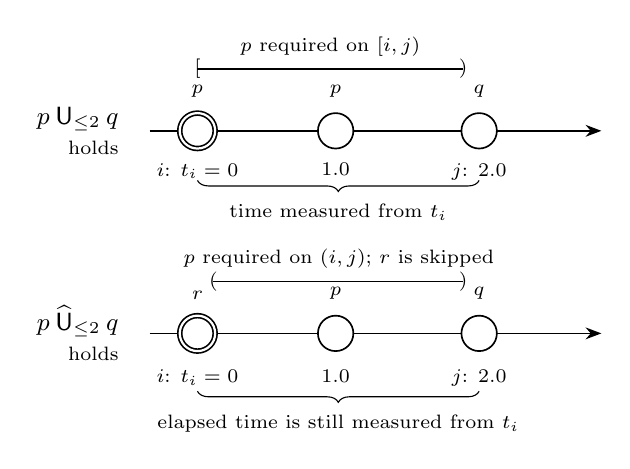
\begin{tikzpicture}[x=1.35cm,y=1.05cm,
  ival/.style={line width=0.5pt},
  ivallab/.style={font=\scriptsize,above=1pt}]
  % Ordinary Until
  \node[anchor=east,font=\small,align=right] at (-0.20,1.30) {$p\Until_{\le 2}q$\\{\scriptsize holds}};
  \draw[fmtimeline] (0,1.30) -- (4.25,1.30);
  \node[fmreference] (u0) at (0.45,1.30) {};
  \node[fmevent] (u1) at (1.75,1.30) {};
  \node[fmevent] (u2) at (3.10,1.30) {};
  \node[above=2pt of u0,font=\scriptsize] {$p$};
  \node[above=2pt of u1,font=\scriptsize] {$p$};
  \node[above=2pt of u2,font=\scriptsize] {$q$};
  \node[below=1.5pt of u0,font=\scriptsize] {$i$: $t_i=0$};
  \node[below=1.5pt of u1,font=\scriptsize] {$1.0$};
  \node[below=1.5pt of u2,font=\scriptsize] {$j$: $2.0$};
  \draw[ival] (0.45,2.05) -- (2.95,2.05);
  \node[font=\scriptsize] at (0.45,2.05) {$[$};
  \node[font=\scriptsize] at (2.95,2.05) {$)$};
  \node[ivallab] at (1.70,2.05) {$p$ required on $[i,j)$};
  \draw[fmbracebottom] (0.45,0.70) -- node[below=5pt,font=\scriptsize] {time measured from $t_i$} (3.10,0.70);

  % Hatted Until
  \node[anchor=east,font=\small,align=right] at (-0.20,-1.15) {$p\hUntil_{\le 2}q$\\{\scriptsize holds}};
  \draw[fmtimeline] (0,-1.15) -- (4.25,-1.15);
  \node[fmreference] (h0) at (0.45,-1.15) {};
  \node[fmevent] (h1) at (1.75,-1.15) {};
  \node[fmevent] (h2) at (3.10,-1.15) {};
  \node[above=2pt of h0,font=\scriptsize] {$r$};
  \node[above=2pt of h1,font=\scriptsize] {$p$};
  \node[above=2pt of h2,font=\scriptsize] {$q$};
  \node[below=3pt of h0,font=\scriptsize] {$i$: $t_i=0$};
  \node[below=3pt of h1,font=\scriptsize] {$1.0$};
  \node[below=3pt of h2,font=\scriptsize] {$j$: $2.0$};
  \draw[ival] (0.60,-0.52) -- (2.95,-0.52);
  \node[font=\scriptsize] at (0.60,-0.52) {$($};
  \node[font=\scriptsize] at (2.95,-0.52) {$)$};
  \node[ivallab] at (1.78,-0.52) {$p$ required on $(i,j)$; $r$ is skipped};
  \draw[fmbracebottom] (0.45,-1.85) -- node[below=5pt,font=\scriptsize] {elapsed time is still measured from $t_i$} (3.10,-1.85);
\end{tikzpicture}

\caption{Ordinary and hatted Until. The double circle is the timing reference.
The hatted operator skips the current event logically but measures from its
timestamp}
\Description{Two timelines with three events each at times 0, 1.0 and 2.0. In the ordinary Until the first event satisfies p and is part of the interval where p is required; in the hatted Until the first event satisfies r and is skipped, p is required only on the later positions, and elapsed time is still measured from the timestamp of the first event, marked by a double circle.}
\label{fig:hatted-until}
\end{figure}

Figure~\ref{fig:hatted-until} contrasts the two readings. The distinction is
useful for sporadicity: if consecutive occurrences of
$e$ must be separated by at least $\theta$, one may write
$\Box(e\Rightarrow\widehat{\Box}_{<\theta}\neg e)$. The hatted form retains
the triggering event as the time origin; ordinary bounded temporal
operators do not express this particular reference shift directly.
Related pointwise MTL constructions and the CASAAL translation are discussed
in prior work~\cite{ouaknine_worrell_lics05,bouyer_chevalier_markey_fsttcs05,li_spin7,casaal_tool}.

\subsection{Timed B\"uchi Automata}
\label{sec:tba}
The verified target is an event-guarded TBA
$\mathcal A=(L,\ell_0,X,E,\mathit{Acc})$. Here $L$ is a finite set of
locations, $\ell_0$ the initial location, $X$ a finite set of clocks,
$E\subseteq L\times\mathsf{Lab}\times\mathsf{Guard}\times 2^X\times L$
is the set of action-labeled transitions with guards and reset sets, and
$\mathit{Acc}\subseteq L$ the B\"uchi set. A run is a sequence
$(\ell_i,v_i)_{i\ge0}$ starting at $\ell_0$; it follows one transition per
event and visits $\mathit{Acc}$ infinitely often. If the selected edge at
event $i$ is $(\ell_i,\alpha_i,g_i,Z_i,\ell_{i+1})$, then the event action
must satisfy $\alpha_i$ and the valuation $v_i$ must satisfy every guard in
$g_i$. There are no location invariants in this model: timing constraints
are checked at the events of the timed word. This is the TBA record
represented in Rocq.

Let $v_i$ be the clock valuation tested at event $i$ and
$\Delta_i=t_{i+1}-t_i$. A transition at event $i$ tests $v_i$ before its
reset decision; the next valuation is
\[
v_{i+1}(x)=
\begin{cases}
\Delta_i,&x\in Z_i,\\
v_i(x)+\Delta_i,&\text{otherwise.}
\end{cases}
\]
The initial nonnegative valuation $v_0$ is existentially quantified, as in
the Rocq clock-consistent-extension semantics; standard zero initialization
is not assumed, and Corollary~\ref{cor:zero-init} shows that it gives the same
language for the translation.

\section{Clocked-LTL Translation}
\label{sec:translation}
\subsection{Shared clock identities}
The translation is structural. It maps Boolean and untimed temporal
operators to their LTL counterparts and maps each primitive timed subformula to an LTL
formula over an extended alphabet. For each action $a$, the extended
alphabet contains distinct action atoms $\mathsf{LAct}(a)$ and
$\mathsf{LNAct}(a)$, as well as clock-related atoms: clock comparisons
$x\sim d$, a reset atom
$\Reset(x)$, and a preservation atom $\Unch(x)$. Under timed-word
interpretation, the action atoms mean that the current action is $a$ or is
different from $a$, respectively. The reset
and preservation atoms describe the clock update at the current event. Clock
values are read before the event's reset, matching the guard semantics of a
timed automaton.

For a formula $f$, let $\Clock(f)$ be its finite set of distinct primitive
hatted timed subformulas. The clock associated with $F\in\Clock(f)$ is
$x=F$ itself. Clock identity uses structural equality on the Rocq MTL syntax
tree. The main result proves that this clock
also serves all dynamic activations of its subformula.
The clock count is therefore bounded by the number of distinct primitive
timed subformulas, which is at most the number of timed occurrences in $f$.
If structural subformulas are represented as shared nodes, the translation
can share their LTL encodings as well; this does not remove the usual
worst-case growth of an LTL-to-B\"uchi construction.

This clock-sharing policy is distinct from automaton-state minimization. The
reset trace is chosen for each formula identity as a whole. In particular,
the proof cannot justify the clock bound
by assigning a fresh clock to each activation and subsequently identifying
those clocks: it establishes directly that a single trace of reset decisions
for the formula is sufficient.

\subsection{Eight primitive clauses}
\label{sec:mtlbuchi}
A path $\pi$ names an occurrence of a subformula in the syntax tree of the
source formula; $\pi0$ and $\pi1$ name its two operands, and $\T(f)$ is the
encoding at the root path. Let $F$ be a primitive hatted formula at path $\pi$,
with operands $p,q$.
Write $x=\mathsf{clock\_of}(F)$, $P=\T_{\pi0}(p)$,
$Q=\T_{\pi1}(q)$, and define
$\alpha\WeakUntil\beta=(\alpha\Until\beta)\lor\Always\alpha$.
For upper comparisons $\precsim\in\{\le,<\}$ and lower comparisons
$\succsim\in\{\ge,>\}$, complements are
$\le^{\mathrm c}=>$, $<^{\mathrm c}=\ge$, $\ge^{\mathrm c}=<$, and
$>^{\mathrm c}=\le$. The four clause shapes give all eight primitive cases:
\begingroup\small
\begin{align}
\T_\pi(p\hUntil_{\precsim d}q)
 &=\Next\bigl(((x\precsim d)\land\Unch(x)\land P)\Until((x\precsim d)\land Q)\bigr),\label{eq:t-hule}\\
\T_\pi(p\hUntil_{\succsim d}q)
 &=\Reset(x)\land\Next\bigl((P\Until((x\succsim d)\land(P\Until Q)))\lor(\Always P\land\Always\Eventually Q)\bigr),\label{eq:t-huge}\\
\T_\pi(p\hRelease_{\precsim d}q)
 &=\Reset(x)\land\Next\bigl(Q\WeakUntil((x\mathrel{\precsim^{\mathrm c}}d)\lor(P\land Q))\bigr),\label{eq:t-hrle}\\
\T_\pi(p\hRelease_{\succsim d}q)
 &=\Next\bigl(((x\mathrel{\succsim^{\mathrm c}}d)\land\Unch(x))\WeakUntil((P\Release Q)\lor((x\mathrel{\succsim^{\mathrm c}}d)\land P))\bigr).
 \label{eq:t-hrge}
\end{align}
\endgroup
The outer $\Next$ implements the hatted shift; $\Reset(x)$ and $\Unch(x)$
encode the restart and preservation choices. The translation uses strong Until for a
bounded witness and weak Until for the Release window. Lower-bounded Until
also has a fairness branch for an obligation whose threshold is delayed
indefinitely. Every clock atom occurs positively, which is the property used
by relaxation in Section~\ref{sec:reset-completion}. The eight local proof
arguments establish the precise behavior in
Section~\ref{subsec:primitive-soundness}.

\subsection{Shared clocks under overlapping activations}
\label{subsec:overlap-motivation}
Hatted operators preserve the triggering timestamp while moving logical
evaluation to the next event. For example,
$\Box(e\Rightarrow\widehat{\Box}_{<\theta}\neg e)$ measures an exclusion
window from the triggering event. The leading next in an ordinary operator
would shift that reference, while omitting it also constrains the triggering
event. Figure~\ref{fig:hat-reference} contrasts these readings.
\begin{figure*}[t]
\centering
\resizebox{\textwidth}{!}{\begin{tikzpicture}[x=1cm,y=1cm,
  tick/.style={line width=0.5pt},
  ticklab/.style={font=\scriptsize,below=1pt},
  verdict/.style={fmnote}]
  % (a) Hatted operator: the intended reading
  \begin{scope}[xshift=0cm]
    \node[font=\small] at (2.4,1.35) {(a) $\Box(e\Rightarrow\widehat{\Box}_{<\theta}\neg e)$};
    \draw[fmtimeline] (0,0) -- (5.0,0);
    \node[fmreference] (a0) at (0.5,0) {};
    \node[fmevent] (a1) at (1.7,0) {};
    \node[fmevent] (a2) at (4.1,0) {};
    \node[above=2pt of a0,font=\scriptsize] {$e$};
    \node[above=2pt of a1,font=\scriptsize] {$a$};
    \node[above=2pt of a2,font=\scriptsize] {$e$};
    \node[verdict] at (4.1,0.78) {satisfied};
    \draw[tick] (3.5,0.12) -- (3.5,-0.12) node[ticklab] {$t_e{+}\theta$};
    \node[ticklab] at (0.5,-0.12) {$t_e$};
    \draw[fmbracebottom] (0.5,-0.62) -- node[below=4pt,fmnote] {$\neg e$ required on $(t_e,t_e{+}\theta)$} (3.5,-0.62);
  \end{scope}

  % (b) Replacing the hat by a leading Next
  \begin{scope}[xshift=5.9cm]
    \node[font=\small] at (2.4,1.35) {(b) $\Box(e\Rightarrow\Next\Box_{<\theta}\neg e)$};
    \draw[fmtimeline] (0,0) -- (5.0,0);
    \node[fmevent] (b0) at (0.5,0) {};
    \node[fmreference] (b1) at (1.7,0) {};
    \node[fmevent] (b2) at (4.1,0) {};
    \node[above=2pt of b0,font=\scriptsize] {$e$};
    \node[above=2pt of b1,font=\scriptsize] {$a$};
    \node[above=2pt of b2,font=\scriptsize] {$e$};
    \node[verdict] at (4.1,0.78) {violated};
    \draw[tick] (3.5,0.12) -- (3.5,-0.12) node[ticklab] {$t_e{+}\theta$};
    \draw[tick] (4.7,0.12) -- (4.7,-0.12) node[ticklab] {$t_a{+}\theta$};
    \node[ticklab] at (1.7,-0.12) {$t_a$};
    \draw[fmbracebottom] (1.7,-0.62) -- node[below=4pt,fmnote] {$\neg e$ required on $[t_a,t_a{+}\theta)$} (4.7,-0.62);
  \end{scope}

  % (c) Dropping the Next
  \begin{scope}[xshift=11.8cm]
    \node[font=\small] at (2.4,1.35) {(c) $\Box(e\Rightarrow\Box_{<\theta}\neg e)$};
    \draw[fmtimeline] (0,0) -- (5.0,0);
    \node[fmreference] (c0) at (0.5,0) {};
    \node[fmevent] (c1) at (1.7,0) {};
    \node[fmevent] (c2) at (4.1,0) {};
    \node[above=2pt of c0,font=\scriptsize] {$e$};
    \node[above=2pt of c1,font=\scriptsize] {$a$};
    \node[above=2pt of c2,font=\scriptsize] {$e$};
    \node[verdict] at (0.5,0.78) {violated at $t_e$};
    \draw[tick] (3.5,0.12) -- (3.5,-0.12) node[ticklab] {$t_e{+}\theta$};
    \node[ticklab] at (0.5,-0.12) {$t_e$};
    \draw[fmbracebottom] (0.5,-0.62) -- node[below=4pt,fmnote] {$\neg e$ required on $[t_e,t_e{+}\theta)$} (3.5,-0.62);
  \end{scope}
\end{tikzpicture}
}
\caption{The hatted sporadicity property (a) and two ordinary-operator
substitutions (b, c) on one finite prefix. Events are labeled by their action;
the marked event is the timing reference, $t_e$ or $t_a$ its timestamp, and the
brace spans the window in which $\neg e$ is required. A leading next (b) shifts
the timing reference to the following event; omitting it (c) includes the
triggering event in the window. The labels satisfied and violated refer to
this prefix}
\Description{Three timelines over the same finite prefix of events. Panel (a) uses the hatted operator and measures the forbidden window from the triggering event. Panels (b) and (c) use ordinary operators, with and without a leading next, and measure the window from the following event or include the triggering event, giving different verdicts on the prefix.}
\label{fig:hat-reference}
\end{figure*}

The proof assigns one clock to each structurally distinct primitive timed
formula, even when that formula is activated repeatedly. The finite prefix in
Table~\ref{tab:overlap-example} illustrates why completeness must account for
all pending obligations: resetting a single clock at the later request can
make an expired earlier deadline appear to be met.
\begin{table}[t]
\centering
\caption{A finite prefix illustrating overlapping response obligations for
$\Box(\mathit{req}\Rightarrow\Diamond_{\le5}\mathit{ack})$, in time units.
Oldest age is the time elapsed since the earliest pending request; reset age
is the value of a single clock reset at each request. Both are read at event
$i$ before any reset at $i$. The acknowledgment at time 6 is late for the
request at time 0 even though its reset age is 2}
\label{tab:overlap-example}
\begin{tabular}{@{}clccc@{}}
\toprule
Event $i$ & Action & Time $t_i$ & Oldest age & Reset age\\
\midrule
0 & $\mathit{req}$ & 0 & 0 & 0\\
1 & $\mathit{req}$ & 4 & 4 & 4\\
2 & $\mathit{ack}$ & 6 & 6 & 2\\
\bottomrule
\end{tabular}
\end{table}
The semantic proof below constructs one trace per
formula-keyed clock and establishes the residual invariants needed when
several activations are pending at once.

\section{From Clocked LTL to a TBA}
\label{sec:tba-construction}
\subsection{LTL-to-B\"uchi contract}
The backend treats the clock-related atoms as independent propositions.
For each action $a$ it receives the atoms $\mathsf{LAct}(a)$ and
$\mathsf{LNAct}(a)$; the contract below constrains only words in which they
are complementary. It returns a propositional B\"uchi automaton
(PBA) whose language, on action-consistent words, is exactly that of the clocked-LTL formula. The theorem is
stated for any such backend, deterministic or not. A propositional word is
\emph{action-consistent} when, at every position, $\mathsf{LNAct}(a)$ holds
exactly when $\mathsf{LAct}(a)$ does not.
\begin{assumption}[Backend correctness]
\label{ass:backend}
An automaton $A$ \emph{meets the contract for} an LTL formula $\Phi$ when, for
every action-consistent propositional word $s$ over the atoms of $\Phi$,
$\mathsf{PBA\_accepts}(A,s)$ iff $s,0\models \Phi$. A backend meets the
contract when, for every formula $\Phi$ it is given, the automaton it returns
meets the contract for $\Phi$.
\end{assumption}
\runinhead{Why a contract.} Stating the backend as an explicit contract keeps the
timed argument independent of the backend. The clocked-LTL formula is an
ordinary untimed LTL formula, so any LTL-to-B\"uchi translator that meets the
contract can be plugged in without touching the rest of the Rocq development.
The tool uses Spot~\cite{spot}, a widely used translator; for this path the guarantee is relative
to the contract. Section~\ref{subsec:verified-backend} proves the contract for a
simple construction, as a witness that the contract can be met, which makes the theorem unconditional. The
timed part of the construction, which is specific to this work, is proved once
and does not depend on which backend is chosen.
This contract ranges over all action-consistent propositional words,
including assignments of the clock-related atoms that do not correspond to any
clock-consistent timed word. Relaxation relies on this scope. 

\subsection{Relaxation and reset completion}
\label{sec:reset-completion}
The propositional backend regards every clock-related atom as independent,
so Assumption~\ref{ass:backend} also covers assignments of these atoms that
cannot arise from any clock-consistent timed trace. Every clock-related atom
in the translation occurs positively, that is, $\T(f)$ is built from these
atoms by $\land$, $\lor$, $\Next$, $\Until$, $\Release$, $\WeakUntil$,
$\Always$ and $\Eventually$ only. Relaxation acts on
each backend transition cube (conjunction of atomic constraints) by removing negative literals over clock
comparisons and reset/preservation markers, removing irrelevant
clock-related literals, and discarding contradictory cubes. Action literals
and positive relevant clock literals are retained. This weakens the cubes
without asking the backend to understand clocks.

Reset completion converts each relaxed cube to a timed transition. Clocks of
upper-bounded hatted Until and lower-bounded hatted Release are preservation
clocks (their clauses use $\Unch$); clocks of lower-bounded hatted Until and
upper-bounded hatted Release are restart clocks (their clauses use $\Reset$). A
preservation clock is reset unless the cube contains $\Unch(x)$; a restart
clock is reset exactly when the cube contains $\Reset(x)$. The markers are
then removed, clock comparisons become guards, and action literals become
labels. The two clock classes move in opposite directions, so the proof
treats them separately.

\begin{lemma}[Reset completion]
\label{lem:reset-completion}
Let an accepting run of the relaxed backend be accompanied by a
clock-consistent extension $\rho$ of its timed word
(Section~\ref{sec:encoding-correctness}). Reset completion
defines a clock-consistent extension $\rho'$ with the same timed word and
the same initial clock valuation. The same state sequence is an accepting
run of the completed TBA on $\rho'$.
\end{lemma}
\begin{proof}
Fix a selected backend cube at position $i$. For a preservation clock $x$,
if the cube contains $\Unch(x)$ then both traces preserve $x$. Otherwise the
completed TBA resets $x$, while $\rho$ may either reset it or preserve it.
Thus the completed reset set contains the original reset decision for $x$.
Induction on positions using the clock recurrence gives
$\CVal_{\rho'}(i,x)\le\CVal_\rho(i,x)$. These clocks occur only in upper
tests ($x\precsim d$), which remain true when the value decreases.

For a restart clock $x$, completion resets it exactly when the cube contains
$\Reset(x)$. A true reset marker requires that $\rho$ resets $x$; without the
marker completion preserves it, whether or not $\rho$ resets it. The
completed reset set is therefore contained in the original one, and the same
induction gives $\CVal_{\rho'}(i,x)\ge\CVal_\rho(i,x)$. These clocks occur
only in lower tests ($x\succsim d$, or their equivalent window-ending
comparisons), which remain true when the value increases. The clock recurrence
holds by the construction of $\rho'$. State transitions, event labels,
guards that remain true, and the B\"uchi accepting set are unchanged, so the
run remains accepting. Rocq proves this result as
\Rocqid{complete_complete}.
\end{proof}

\subsection{Worked example: bounded eventuality with an exclusion window}
Let
\[
  f=(\Diamond_{\le5}p)\land(\Box_{<2}\neg p).
\]
It requires $p$ to be false at every position before age 2 and to hold at
some position no later than age 5. Figure~\ref{fig:translation-reference-tba} shows a hand-simplified
equivalent one-clock TBA, not the syntax-directed output, since the latter assigns
separate clocks to the two distinct timed subformulas. The steps below show
the clocked-LTL translation and timed reinterpretation. The concrete instance
checked in Rocq is the alarm-response example in
Section~\ref{sec:alarm-example}.

\begin{figure}[t]
\centering
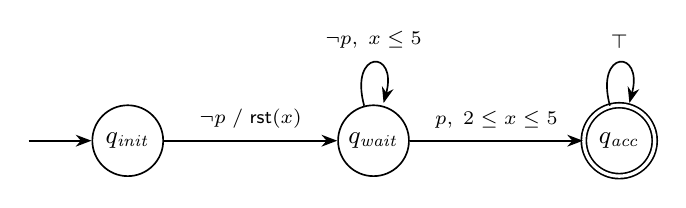
\begin{tikzpicture}[node distance=22mm]
  \node[fmstate] (q0) {$q_{\mathit{init}}$};
  \node[fmstate,right=of q0] (q1) {$q_{\mathit{wait}}$};
  \node[fmaccept,right=of q1] (q2) {$q_{\mathit{acc}}$};
  \draw[fmedge] ([xshift=-8mm]q0.west) -- (q0.west);
  \draw[fmedge] (q0) -- node[fmlabel,above,yshift=3pt] {$\neg p\;/\;\mathsf{rst}(x)$} (q1);
  \draw[fmedge] (q1) edge[loop above] node[fmlabel,yshift=4pt] {$\neg p,\;x\le5$} (q1);
  \draw[fmedge] (q1) -- node[fmlabel,above,yshift=3pt] {$p,\;2\le x\le5$} (q2);
  \draw[fmedge] (q2) edge[loop above] node[fmlabel,yshift=4pt] {$\top$} (q2);
\end{tikzpicture}

\caption{Hand-simplified equivalent event-guarded TBA for $f$. Edges are labeled by
event and guard; $\mathsf{rst}(x)$ resets $x$, and $q_{\mathit{acc}}$ is the
accepting location. The initial transition requires $\neg p$ and resets $x$;
the edges leaving the waiting location are guarded by $x\le5$, and the edge to
the accepting location also requires $x\ge2$. Thus $p$ first holds at an age
in $[2,5]$}
\Description{A small event-guarded timed Büchi automaton with an initial transition that resets a clock, a waiting location with edges guarded by a clock at most 5, and an accepting location reached by an edge that also requires the clock to be at least 2.}
\label{fig:translation-reference-tba}
\end{figure}

\begin{enumerate}[label=Step~\arabic*:,leftmargin=*]
\item The formula is in negation normal form. Expanding the derived operators
and applying the timed-operator identities gives
\[
\begin{aligned}
f
 &= (\top\Until_{\le5}p)\land(\bot\Release_{<2}\neg p)\\
 &= \bigl(p\lor(\top\land\top\hUntil_{\le5}p)\bigr)\\
 &\qquad\land\bigl(\neg p\land(\bot\lor\bot\hRelease_{<2}\neg p)\bigr).
\end{aligned}
\]
These current-position cases follow Eqs.~\eqref{eq:derive-ule} and
\eqref{eq:derive-rle}.

\item The two distinct primitive timed subformulas receive clocks $x$ and
$y$, respectively. Their clocked-LTL translation is
\begingroup\small
\begin{align*}
\Phi_U={}&p\lor\bigl(\top\land\Next\bigl(((x\le5)\land\Unch(x)\land\top)\Until((x\le5)\land p)\bigr)\bigr),\\[-1mm]
\Phi_R={}&\neg p\land\bigl(\bot\lor(\Reset(y)\land\Next(\neg p\WeakUntil((y\ge2)\lor(\bot\land\neg p))))\bigr),\\[-1mm]
\T(f)={}&\Phi_U\land\Phi_R.
\end{align*}
\endgroup
The Until clause preserves $x$; the Release test $y\ge2$ complements the source
bound $<2$, allowing $p$ from age 2.

\item The Spot~2.16 graph for $\T(f)$ is redrawn at the top of
Figure~\ref{fig:translation-steps45}. The clock guards $x\le5$ and
$y\ge2$, the markers $\mathsf{unch}(x)$ and $\mathsf{rst}(y)$, and the action
atom $p$ are propositions to the backend. The graph has four
states and seven transitions.

\item Relaxation removes negative literals over extended clock atoms, here
$\neg(y\ge2)$. Reset completion resets the preservation clock $x$ unless
$\mathsf{unch}(x)$ is present; the restart clock $y$ is reset exactly when
$\mathsf{rst}(y)$ is present. The bottom of
Figure~\ref{fig:translation-steps45} shows the same state graph after these
operations: each edge carries the event, the clock guard, and the resets. The
event is an action ($p$ or $\neg p$), and $\top$ stands for any event.
Relaxation removes $\neg(y\ge2)$ from the loop on~2, which therefore stays
enabled after age~2. From then on state~2 behaves as state~3, since $y$ is
never reset again, so no word is added; the two states could be merged, which
the translation does not do.
\end{enumerate}

\begin{figure*}[!t]
\centering
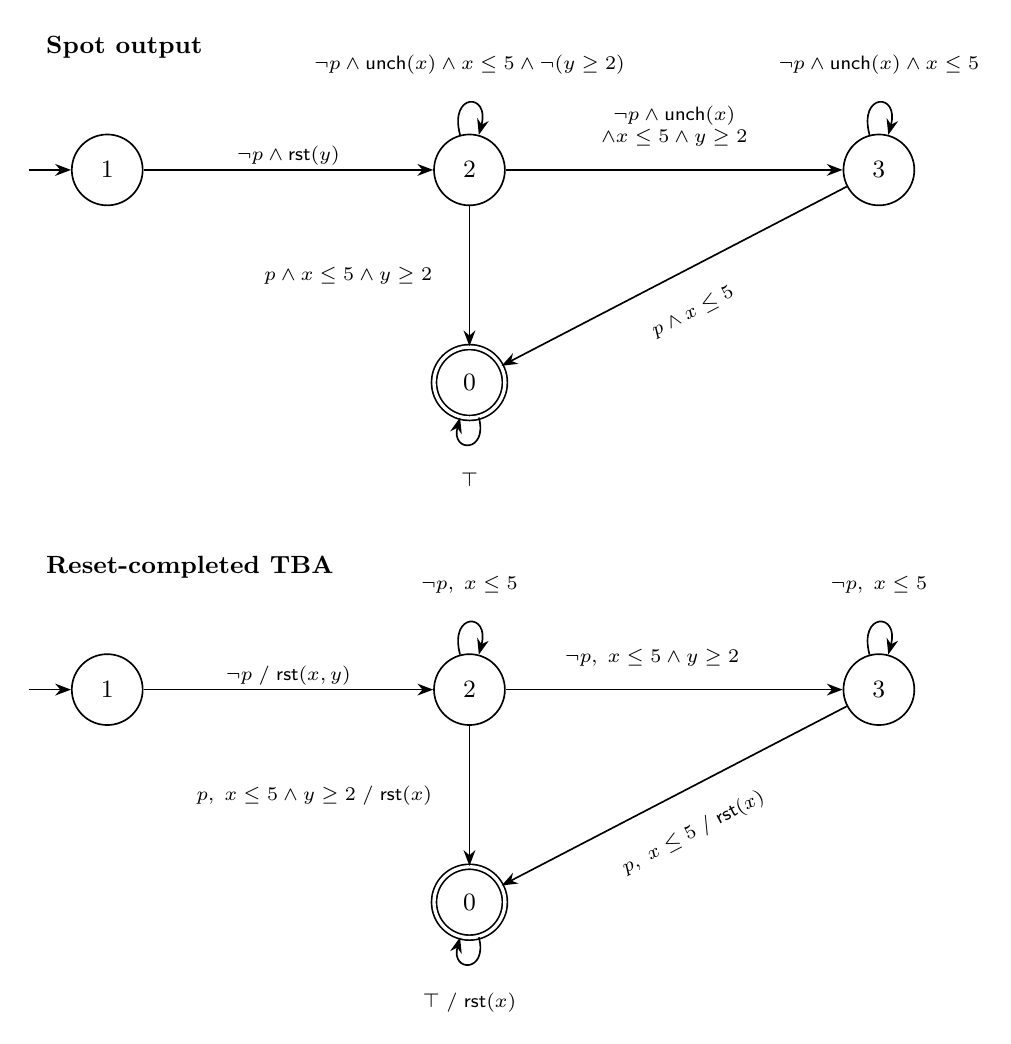
\begin{tikzpicture}[x=1cm,y=1cm]
% Left: the saved Spot graph for T(f) (negated event atom printed as !"p").
% Right of the arrows: guards and resets of the reset-completed TBA.
\begin{scope}[xshift=0cm]
  \node[fmnote,font=\small\bfseries,anchor=west] at (-0.9,1.55) {Spot output};
  \node[fmstate] (a0) at (0.0,0.0) {$1$};
  \node[fmstate] (a1) at (4.6,0.0) {$2$};
  \node[fmstate] (a3) at (9.8,0.0) {$3$};
  \node[fmaccept] (a2) at (4.6,-2.7) {$0$};
  \draw[fmedge] (-1.0,0.0) -- (a0);
  \draw[fmedge] (a0) -- node[fmlabel,above] {$\neg p\land\mathsf{rst}(y)$} (a1);
  \draw[fmedge] (a1) edge[loop above,looseness=6]
    node[fmlabel,yshift=9pt] {$\neg p\land\mathsf{unch}(x)\land x\le5\land\neg(y\ge2)$} (a1);
  \draw[fmedge] (a1) -- node[fmlabel,above,yshift=7pt,xshift=0pt] {$\neg p\land\mathsf{unch}(x)$\\$\land x\le5\land y\ge2$} (a3);
  \draw[fmedge] (a1) -- node[fmlabel,left,xshift=-12pt] {$p\land x\le5\land y\ge2$} (a2);
  \draw[fmedge] (a3) edge[loop above,looseness=6]
    node[fmlabel,yshift=9pt] {$\neg p\land\mathsf{unch}(x)\land x\le5$} (a3);
  \draw[fmedge] (a3) -- node[fmlabel,sloped,below,yshift=-10pt] {$p\land x\le5$} (a2);
  \draw[fmedge] (a2) edge[loop below,looseness=5] node[fmlabel,yshift=-9pt] {$\top$} (a2);
\end{scope}

\begin{scope}[yshift=-6.6cm]
  \node[fmnote,font=\small\bfseries,anchor=west] at (-0.9,1.55) {Reset-completed TBA};
  \node[fmstate] (b0) at (0.0,0.0) {$1$};
  \node[fmstate] (b1) at (4.6,0.0) {$2$};
  \node[fmstate] (b3) at (9.8,0.0) {$3$};
  \node[fmaccept] (b2) at (4.6,-2.7) {$0$};
  \draw[fmedge] (-1.0,0.0) -- (b0);
  \draw[fmedge] (b0) -- node[fmlabel,above] {$\neg p\;/\;\mathsf{rst}(x,y)$} (b1);
  \draw[fmedge] (b1) edge[loop above,looseness=6]
    node[fmlabel,yshift=9pt] {$\neg p,\;x\le5$} (b1);
  \draw[fmedge] (b1) -- node[fmlabel,above,yshift=7pt,xshift=-8pt] {$\neg p,\;x\le5\land y\ge2$} (b3);
  \draw[fmedge] (b1) -- node[fmlabel,left,xshift=-12pt] {$p,\;x\le5\land y\ge2\;/\;\mathsf{rst}(x)$} (b2);
  \draw[fmedge] (b3) edge[loop above,looseness=6]
    node[fmlabel,yshift=9pt] {$\neg p,\;x\le5$} (b3);
  \draw[fmedge] (b3) -- node[fmlabel,sloped,below,yshift=-10pt] {$p,\;x\le5\;/\;\mathsf{rst}(x)$} (b2);
  \draw[fmedge] (b2) edge[loop below,looseness=5] node[fmlabel,yshift=-9pt] {$\top\;/\;\mathsf{rst}(x)$} (b2);
\end{scope}
\end{tikzpicture}

\caption{The Spot~2.16 graph for $\T(f)$ (top, redrawn; the labels are
propositional cubes over the action atom $p$, the clock guards, and the markers
$\mathsf{unch}(x)$ and $\mathsf{rst}(y)$) and the reset-completed TBA obtained
from it by hand (bottom; same state numbers, which are Spot's). A TBA edge is labeled
by the event, the clock guard, and, after a slash, the clocks reset; $\top$ is
any event, and an edge without a slash resets no clock. This graph-to-TBA
illustration is not the formally verified alarm-response backend instance}
\Description{Two automata with the same state numbers. The top one is Spot's graph for the clocked-LTL formula, with edges labeled by propositional cubes. The bottom one is the reset-completed timed automaton derived from it, with edges labeled by event, clock guard, and resets after a slash.}
\label{fig:translation-steps45}
\end{figure*}


\section{Mechanized Correctness}
\label{sec:correctness}
\label{sec:encoding-correctness}
For a formula $f$, an extended word $\rho$ augments the timed word with a
nonnegative value $\CVal_\rho(i,x)$ and a reset decision
$\CReset_\rho(i,x)$ for every formula-keyed clock $x\in\Clock(f)$ at each
position $i$. It is clock-consistent when, with
$\Delta_i=t_{i+1}-t_i$,
\begin{equation}
\CVal_\rho(i+1,x)=
\begin{cases}
\Delta_i,&\CReset_\rho(i,x),\\
\CVal_\rho(i,x)+\Delta_i,&\text{otherwise.}
\end{cases}
\label{eq:clock-update}
\end{equation}
The value at $i$ is tested before the reset decision at $i$.
Over an extended word, the clocked-LTL atoms are interpreted as follows:
$(x\sim d)$ holds at $i$ iff $\CVal_\rho(i,x)\sim d$; $\Reset(x)$ holds at $i$
iff $\CReset_\rho(i,x)$; $\Unch(x)$ holds at $i$ iff $\neg\CReset_\rho(i,x)$;
and $\mathsf{LAct}(a)$, $\mathsf{LNAct}(a)$ hold at $i$ iff the action at $i$
is, respectively is not, $a$. The relation
$\mathsf{same\_base}(\rho,w)$ means that the projection of $\rho$ onto actions
and timestamps gives $w$.

\subsection{Soundness for arbitrary reset traces}
\label{subsec:primitive-soundness}
The soundness direction does not select or assume any particular reset
policy; in particular, it does not use the canonical policy that
Section~\ref{subsec:canonical-policy} defines for completeness. For
each primitive formula $F$ at path $\pi$, the corresponding Rocq lemma
\texttt{sound\_*} turns $\rho,i\satL\T_\pi(F)$ into
$\ewbase(\rho),i\satM F$, assuming clock consistency and
induction hypotheses for its operands. 
Clock consistency gives two useful bounds. If a clock is preserved on
$[i,j)$, then
\[
\CVal_\rho(j,x)=\CVal_\rho(i,x)+\elapsed_w(i,j).
\]
Since clock values are nonnegative, preservation implies
$\CVal_\rho(j,x)\ge\elapsed_w(i,j)$. If it is reset at $i$, then for every
$j\ge i+1$,
\[
\CVal_\rho(j,x)\le\elapsed_w(i,j),
\]
with equality when it is not reset again before $j$. The upper-guard
implication follows from the first inequality; the lower-guard implication
follows from the second. Both follow by induction from
Eq.~\eqref{eq:clock-update} and nonnegative delays.

\runinhead{Upper-bounded hatted Until.}
The outer $\Next$ moves to the first strictly future event. The strong Until
then supplies a witness $j>i$ satisfying $Q$, with $P$ at every intermediate
event and $\Unch(x)$ throughout that prefix. Regardless of whether the clock
was reset at $i$, its value at $i+1$ is at least $\Delta_i$.
Preservation after $i+1$ therefore gives
\[
\CVal_\rho(j,x)\ge
\Delta_i+\elapsed_w(i+1,j)=\elapsed_w(i,j).
\]
The endpoint guard $x\le d$ implies $\elapsed_w(i,j)\le d$; the guard $x<d$
implies $\elapsed_w(i,j)<d$. Induction on $P,Q$ yields the hatted Until
witness and prefix in both cases. The strong Until is essential: an infinite
continuation with no $Q$ endpoint is not a bounded Until witness.

\runinhead{Lower-bounded hatted Until.}
Here the translation requires $\Reset(x)$ at $i$. The finite branch (the first disjunct of
Eq.~\eqref{eq:t-huge}) waits for a position with $x\succsim d$ and then supplies an
ordinary $P\Until Q$ witness. Since subsequent resets can only make a clock
younger, $\CVal_\rho(j,x)\le\elapsed_w(i,j)$; thus the threshold guard implies
the required lower-bound comparison. The nested Until supplies $P$ up to the
$Q$ witness. The other branch is
$\Always P\land\Always\Eventually Q$. It gives an unbroken $P$ prefix and
unboundedly many $Q$ positions; divergence of timestamps lets us choose a
$Q$ witness beyond any finite lower bound. For the strict case, choose a
recurring $Q$ at distance at least $d+1$ from $i+1$. Since
$t_i\le t_{i+1}$, that same event is strictly more than $d$ after $i$. This is
the additional argument in \Rocqid{sound_UhatGt}; it preserves the strict
boundary.

\runinhead{Upper-bounded hatted Release.}
The translation resets the clock at $i$ and uses weak Until with $Q$ as its
left condition. Consequently, $Q$ holds at each future event until either
$P\land Q$ discharges the Release obligation or the complementary clock test
marks the end of the upper window. For a non-strict upper bound, the window
ends at $x>d$; for a strict upper bound, it ends at $x\ge d$. If the clock
has been reset again, its value is no larger than the elapsed time from $i$,
so either endpoint guard can hold only after the corresponding physical-time
window has ended. If weak Until ends at $P\land Q$, $P$ at that earlier event
discharges later Release obligations. Both comparisons are thus proved with
their exact strict boundary.

\runinhead{Lower-bounded hatted Release.}
Before the threshold, the left side of weak Until requires both the
pre-threshold comparison and $\Unch(x)$. Thus an arbitrary reset trace
cannot move the clock backwards while the pre-threshold condition remains
active. Once the comparison becomes false, the translation requires ordinary
$P\Release Q$ from that event, unless the right-side alternative has already
terminated the obligation at a position satisfying $P$ while still below the
threshold. An older initial clock value can make the translation enter the
ordinary Release branch earlier than the MTL interval does; this only imposes
a stronger condition. 

The standard LTL semantics used here are formalized in Rocq as
\Rocqid{LG_semantics}, \Rocqid{LGF_semantics},
\Rocqid{LW_semantics}, and \Rocqid{LF_semantics}. Time divergence is used
only for the fairness witness in lower-bounded Until; no assumption on the
reset policy beyond clock consistency is used in any soundness family.

\subsection{Canonical reset policy and residual obligations}
\label{subsec:canonical-policy}
Completeness must choose one clock trace for each primitive formula, even
when activations overlap. The canonical policy preserves a reference only
while its residual obligation is still useful. Recall that
$\elapsed_w(i,j)=t_j-t_i$. For upper-bounded Until define
\begin{align}
\mathsf{URes}_{\precsim}(i,v,d,p,q)\iff{}
&\exists j\ge i.\;v+\elapsed_w(i,j)\precsim d\nonumber\\[-1mm]
&\land w,j\satM q\nonumber\\[-1mm]
&\land\forall k\in[i,j).\,w,k\satM p\label{eq:ures-le}
\end{align}
The residual says that a $q$ endpoint is still reachable with the current
clock age and the required $p$ prefix. For lower-bounded Release define
\begin{align}
\mathsf{RRes}_{\succsim}(i,v,d,p,q)\iff{}
&\forall j\ge i.\;v+\elapsed_w(i,j)\succsim d\Rightarrow\nonumber\\[-1mm]
&\Bigl(w,j\satM q~\lor\nonumber\\[-1mm]
&\exists k\in[i,j).\,w,k\satM p\Bigr)\label{eq:rres-ge}
\end{align}
The residual $\mathsf{RRes}$ is universal: every position already beyond the
threshold must have $q$ or an earlier $p$ that discharges the obligation;
$\mathsf{URes}$ is its existential counterpart (a reachable $q$ endpoint).

For a clock $x=F$, let $v=\CVal_{\rho^\star}(i,x)$; Table~\ref{tab:canonical-policy} gives the
policy.
\begin{table}[t]
\centering
\caption{Canonical reset decision at position $i$, with
$v=\CVal_{\rho^\star}(i,x)$, $\precsim$ ranging over $\{\le,<\}$ and
$\succsim$ over $\{\ge,>\}$. A decision ``Preserve iff $C$'' means that the
clock is preserved when $C$ holds and reset otherwise; ``Reset iff $C$'' means
the converse. $\mathsf{URes}$ and $\mathsf{RRes}$ are defined in
Eqs.~\eqref{eq:ures-le} and~\eqref{eq:rres-ge}}
\label{tab:canonical-policy}
\begin{tabular}{@{}p{0.35\columnwidth}p{0.59\columnwidth}@{}}
\toprule
Primitive formula $F$ & Decision at $i$\\
\midrule
$p\hUntil_{\precsim d}q$ &
Preserve iff $v\precsim d$, $\mathsf{URes}_{\precsim}(i,v,d,p,q)$, and
$w,i\not\satM q$.\\
$p\hUntil_{\succsim d}q$ and $p\hRelease_{\precsim d}q$ &
Reset iff $w,i\satM F$.\\
$p\hRelease_{\succsim d}q$ &
Preserve iff $v\not\succsim d$, $\mathsf{RRes}_{\succsim}(i,v,d,p,q)$, and
$w,i\not\satM p$.\\
\bottomrule
\end{tabular}
\end{table}
The resulting values begin at $u_0=0$ and evolve by
\[
u_{i+1}=
\begin{cases}
\Delta_i,&\text{if the policy resets at }i,\\
u_i+\Delta_i,&\text{otherwise.}
\end{cases}
\]
This is a word-dependent completeness witness, not a reset algorithm in an
executable translator. Its decisions are keyed by the primitive formula
itself, not by an occurrence path.

\runinhead{A worked trace.}
Let $F=\top\hUntil_{\le5}\mathit{ack}$, so $d=5$ and $p=\top$, and let the word
have events $\mathit{req}$ at time $0$, $\mathit{req}$ at time $2$, and
$\mathit{ack}$ at time $4$ (positions $0$, $1$, $2$), so that $\Delta_0=2$ and
$\Delta_1=2$. Then $w,0\satM F$ and $w,1\satM F$, since the acknowledgment lies
within $5$ time units of both. The canonical policy gives:
\begin{itemize}
  \item $i=0$: $v=u_0=0\le5$; $\mathsf{URes}$ holds with witness $j=2$, because
        $0+(4-0)\le5$ and $\mathit{ack}$ holds at $2$; and $w,0\not\satM\mathit{ack}$. The clock
        is \emph{preserved}, so $u_1=0+2=2$.
  \item $i=1$: the second request is a new activation of $F$ but does not reset
        the clock. We have $v=u_1=2\le5$; $\mathsf{URes}$ holds with $j=2$, because
        $2+(4-2)\le5$; and $w,1\not\satM\mathit{ack}$. The clock is preserved,
        so $u_2=4$.
  \item $i=2$: $v=4\le5$, but $w,2\satM\mathit{ack}$, so the policy resets.
\end{itemize}
At the witness position the single clock reads $4\le5$, which is the age of the
\emph{older} activation, since the clock was not reset at the second request.
The younger activation, whose own age is $2$, is served by the same reading,
because the older age is larger and still within the bound. Compare
Table~\ref{tab:overlap-example}, where the acknowledgment is late for the older
request: there $\mathsf{URes}$ already fails at position $0$ and no trace is
needed. The preservation test $\mathsf{URes}$ keeps the reference only while
the obligation is still satisfiable.

\subsection{Completeness for one canonical trace}
\label{subsec:primitive-completeness}
For every formula satisfied by $w$, completeness constructs one clock-consistent
extension $\rho^\star$ that serves all activations of every shared clock.
The four operator families use different invariants:

\runinhead{Upper-bounded hatted Until.}
Choose the first witness $j>i$ of the formula at $i$, that is, the first
position at which $q$ holds within the bound with $p$ on $(i,j)$, while
the activation remains pending. The
key invariant along the translated strong-Until prefix is
\begin{equation}
\CVal_{\rho^\star}(n,x)+\elapsed_w(n,j)\le d
\quad(i<n\le j).
\label{eq:canonical-until-invariant}
\end{equation}
For $<d$, replace $\le d$ by $<d$. The invariant need not hold at $i$:
the translation begins with $\Next$, so the first clock test is at $i+1$.
If the policy resets at $i$, then $u_{i+1}=\Delta_i$ and
$u_{i+1}+\elapsed_w(i+1,j)=\elapsed_w(i,j)$, which is within the bound for
the chosen witness. If it preserves at $i$, the residual supplies a still
reachable $q$ endpoint and $p$ prefix; because the current $q$ has not
discharged that residual, its witness is strictly after $i$, and the same
identity advances the residual inequality to $i+1$. Because $j$ is the first such
position, $q$ fails at every intermediate position $n$ with $i<n<j$: otherwise
$n$ would be an earlier witness, since $p$ holds on $(i,n)\subseteq(i,j)$. The
invariant gives $\CVal_{\rho^\star}(n,x)+\elapsed_w(n,j)\le d$, so
$\mathsf{URes}_{\le}$ holds at $n$ with witness $j$. Hence the policy preserves
the reference at every intermediate position, which is what the conjunct
$\Unch(x)$ of the translation requires; the endpoint $j$ satisfies $q$ and the
clock comparison. A reference reset earlier has a larger age than any later
one, so if it still reaches the shared endpoint within $d$, the obligations of
the later activations are covered as well. This is the invariant proved
by \Rocqid{complete_UhatLe} and \Rocqid{complete_UhatLt}.

\runinhead{Lower-bounded hatted Until.}
Whenever the formula is true at an activation, the policy resets its clock.
Starting from $i+1$, a first position at which the canonical clock reaches
$d$ (or strictly exceeds $d$) and has a qualifying later $q$ witness gives
the finite branch (the first disjunct of Eq.~\eqref{eq:t-huge}): the clock guard supplies the lower-bound
test, and the nested $P\Until Q$ supplies the remaining witness. Before the
first such position, the proof maintains an active-witness invariant. At
each $n\ge i+1$ it supplies an activation $s<n$, a witness $m\ge n$ with
$t_m-t_s\ge d$ and $w,m\models q$, $p$ at every intermediate position, and
$\CVal_{\rho^\star}(n,x)=t_n-t_s$. Since $n$ precedes the first qualifying position, $n<m$; thus $p$ holds at
$n$ and a $q$ witness
remains at or after every $n$. If a first qualifying position occurs, the
finite branch applies; if none occurs, the invariant yields
$\Always P\land\Always\Eventually Q$, the fairness branch (the second disjunct of Eq.~\eqref{eq:t-huge}).
Divergence converts recurring $q$ positions into a witness beyond the
lower bound. These are the arguments
formalized by \Rocqid{complete_UhatGe} and \Rocqid{complete_UhatGt}.

\runinhead{Upper-bounded hatted Release.}
At every activation where the hatted Release formula is true, the policy
resets the restart clock. If the first future event lies inside the bounded window, it must satisfy $q$,
as required by the hatted Release semantics; otherwise the stopping guard
already holds there and the weak Until is discharged. The universal condition then
continues as weak Until: $q$ holds until either $p\land q$ discharges all
later points or the clock passes the end of the bounded window. For a
$\le d$ window the stopping guard is $x>d$; for a $<d$ window it is
$x\ge d$. Resetting at a later true activation can extend the clock window,
but the later formula's truth supplies the corresponding future
$q$-or-discharge condition. Thus a single reset trace satisfies both the old
and new obligations. These are the arguments formalized by
\Rocqid{complete_RhatLe} and \Rocqid{complete_RhatLt}.

\runinhead{Lower-bounded hatted Release.}
While $\mathsf{RRes}_{\ge}$ holds, $v<d$, and $p$ has not discharged the
obligation, the policy preserves the clock. Preservation advances both the
clock and the residual by
\[
(i,v)\longmapsto(i+1,v+\Delta_i),
\qquad
\elapsed_w(i,j)=\Delta_i+\elapsed_w(i+1,j).
\]
Substitution in Eq.~\eqref{eq:rres-ge} proves
$\mathsf{RRes}_{\ge}(i+1,v+\Delta_i,d,p,q)$. The instance $\succsim\,=\,>$
gives the same shift for $\mathsf{RRes}_{>}$ when $v\le d$. The residual ensures that
every event in the already-entered lower-bound region has $q$ or an earlier
$p$. If $p$ occurs while the clock is still below threshold, the right side
of weak Until terminates with that $p$; otherwise the clock reaches the
threshold and the residual supplies the ordinary Release continuation.
For $\ge d$, an event exactly at $d$ is already in the constrained region;
for $>d$, the prefix includes equality and only a strictly later event
starts the region. The corresponding proofs are
\Rocqid{complete_RhatGe}, \Rocqid{rge_residual_shift},
\Rocqid{complete_RhatGt}, and \Rocqid{rgt_residual_shift}.

\subsection{Occurrence-indexed structural induction}
\label{subsec:occurrence-induction}
The completeness proof must recurse through a syntax tree while preserving
the root formula's clock identities. Write
$\mathsf{node}(root,\pi)=f$ when the path lookup at $\pi$ in $root$
returns $f$ (the Rocq notation is
\texttt{node\_at root pi = Some f}). Let
$\rho^\star=\mathsf{canonical\_ext}(root,w)$. The strengthened theorem is:
\begin{theorem}[Canonical correctness at every syntactic occurrence]
\label{thm:canonical-all}
For every well-formed root formula, every path $\pi$ with
$\mathsf{node}(root,\pi)=f$, and every position $i$,
\[
w,i\satM f
\quad\Longleftrightarrow\quad
\rho^\star,i\satL\T_\pi(f).
\]
The same extension $\rho^\star$ is constructed once from $root$ and $w$ and
is used for all paths.
\end{theorem}
\begin{proof}
Proceed by structural induction on $f$. Boolean and untimed temporal cases
follow from their semantics and the induction hypotheses. For a binary
constructor, \Rocqid{node_at_left_binary} and
\Rocqid{node_at_right_binary} locate the child formulas at the extended
paths. Ordinary timed operators unfold to the derived Boolean/hatted
definitions, leaving the eight primitive cases proved above. In each hatted
case, the forward direction uses its canonical-completeness lemma and the
reverse direction its policy-independent soundness lemma. The path locates
the formula for induction; it is not part of the clock key. The Rocq theorem
is \Rocqid{canonical_encoding_all}.
\end{proof}

Clock identity is structural equality of the primitive formula value,
including constructor, operands, comparison, and real bound. Hence if
$\mathsf{node}(root,\pi_1)=F=\mathsf{node}(root,\pi_2)$ for a primitive
timed formula, both paths refer to the same clock and the same canonical
trace. Rocq proves this as \Rocqid{identical_nodes_share_clock} and
\Rocqid{identical_nodes_share_canonical_trace}. The theorem therefore
uses one extension for the entire root formula, not a separate witness per
occurrence or activation.

\subsection{Clocked-LTL correctness and TBA composition}
\begin{theorem}[Correctness of the clock encoding]
\label{thm:encoding-correctness}
For every well-formed formula $f$ and timed word $w$,
\begin{align*}
w,0\satM f\quad\Longleftrightarrow\quad
\exists\rho.\;&\mathsf{same\_base}(\rho,w)\\[-1mm]
&\land\mathsf{clock\_consistent}(\rho)\\[-1mm]
&\land\rho,0\satL\T(f).
\end{align*}
\end{theorem}
This is \Rocqid{EncodingCorrect_proved}. Its left-to-right direction uses
the one canonical extension of Theorem~\ref{thm:canonical-all} at the root
path. Its right-to-left direction uses the soundness induction for an
arbitrary extension $\rho$; completeness cannot be used to reason about an
arbitrary reset trace. Thus the quantifiers differ: soundness holds
for every consistent satisfying extension, whereas completeness constructs a
single one.

\begin{corollary}[One clock per distinct primitive timed subformula]
\label{cor:one-clock-formula}
All occurrences of the same primitive timed formula use the same clock, and
the encoding uses exactly the clocks in $\Clock(f)$. The clock count is
independent of the number of syntax-tree occurrences and dynamic activations.
\end{corollary}
\begin{proof}
The translation is indexed by elements of $\Clock(f)$, while
\Rocqid{T_uses_every_clock} proves that each such clock occurs in $\T(f)$.
The canonical trace of Theorem~\ref{thm:canonical-all} serves every activation
of that formula.
\end{proof}

For a propositional B\"uchi automaton $A$ over the extended atoms, let
$\mathsf{compile\_with}(A)$ denote relaxation followed by reset completion.
Its correctness contract is Assumption~\ref{ass:backend}. The single composed
theorem (Figure~\ref{fig:correctness-composition}), for any backend that meets
that contract, is:
\begin{theorem}[MTL-to-TBA correctness for a backend meeting the contract]
\label{thm:mtl-to-tba-correct}
For every well-formed formula $f$, timed word $w$, and propositional
B\"uchi automaton $A$ satisfying Assumption~\ref{ass:backend},
\[
w,0\satM f
\quad\Longleftrightarrow\quad
\mathsf{TBA\_accepts}(\mathsf{compile\_with}(A),w).
\]
In Rocq this is \Rocqid{MTL_to_TBA_correct_with}.
\end{theorem}
\begin{proof}
For the forward direction, the encoding theorem supplies a canonical clock-consistent
extension satisfying $\T(f)$. The backend contract gives an accepting
propositional run. Relaxation carries the run to the relaxed automaton by
\Rocqid{relax_complete}; reset completion then supplies the completed
clock-consistent extension and accepting TBA run by
\Rocqid{complete_complete}.

For the converse direction, an accepting completed run first projects to a run of the
relaxed backend by \Rocqid{complete_sound}. Call an extended atom
\emph{relevant} if it occurs in $\T(f)$. At each position, reconstruct a
propositional valuation $s'$ satisfying the selected original backend cube: $s'$
takes its action atoms and its irrelevant atoms from the cube (a cube that does
not mention an irrelevant atom leaves it arbitrary), makes true exactly the
relevant extended atoms that occur positively in the surviving cube, and makes
every other relevant extended atom false. In particular, deleted negative
literals are false in $s'$. The same state sequence remains accepting. The
backend contract gives $\T(f)$ on $s'$. The word of the relaxed run agrees with
$s'$ on action atoms and is true on every relevant extended atom that is true in
$s'$, so positivity of $\T(f)$ transfers satisfaction to the relaxed word, as formalized by
\Rocqid{relax_sound}. Applying the soundness direction of
Theorem~\ref{thm:encoding-correctness} gives $w,0\satM f$.
\end{proof}

\begin{corollary}[Zero-initialized clocks]
\label{cor:zero-init}
Under the hypotheses of Theorem~\ref{thm:mtl-to-tba-correct}, $w,0\satM f$
holds if and only if $\mathsf{compile\_with}(A)$ accepts $w$ with every clock
starting at 0, that is, by a clock-consistent extension $\rho$ with
$\CVal_\rho(0,x)=0$ for every clock $x$. For this translation, zero and
existentially chosen initial clock values therefore define the same language.
In Rocq this is \Rocqid{MTL_to_TBA_correct_with_zero_init}.
\end{corollary}
\begin{proof}
A run with zero initial clocks is a run with some initial clock values, so the
converse direction is Theorem~\ref{thm:mtl-to-tba-correct}. For the forward
direction, the canonical extension of Theorem~\ref{thm:canonical-all} starts
every clock at 0. The backend step and relaxation do not involve clocks, and
reset completion keeps the initial valuation of the extension it starts from
(\Rocqid{complete_complete_init}, the proof of \Rocqid{complete_complete} with
this conclusion added). The completed TBA therefore accepts $w$ from the zero
valuation. The corollary is a property of this translation; it does not hold
for arbitrary TBAs.
\end{proof}

\begin{figure*}[!t]
\centering
\resizebox{\textwidth}{!}{%
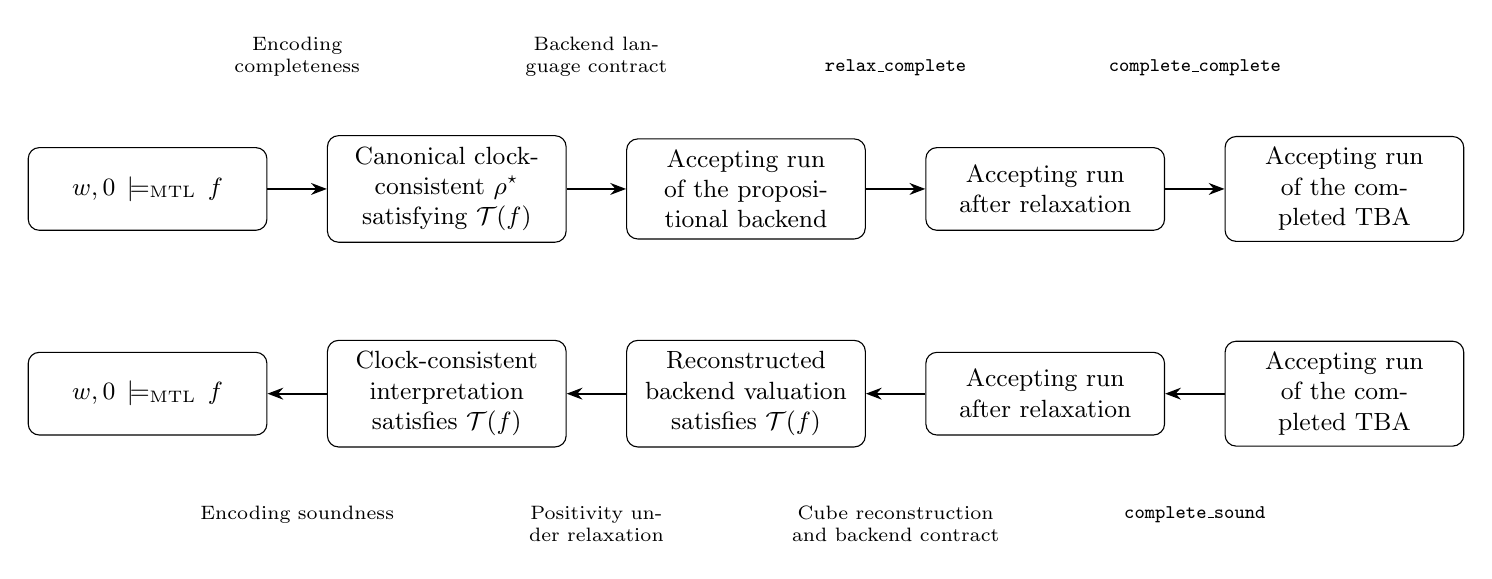
\begin{tikzpicture}[
  proofbox/.style={draw,rounded corners,align=center,text width=2.75cm,
    minimum height=1.05cm,font=\small,inner sep=4pt},
  flow/.style={-{Stealth[length=2mm]},thick},
  flowlabel/.style={font=\scriptsize,align=center,text width=2.65cm}
]
\node[proofbox] (mtl) at (0,0) {$w,0\satM f$};
\node[proofbox] (enc) at (3.8,0) {Canonical clock-consistent
  $\rho^\star$ satisfying $\T(f)$};
\node[proofbox] (pb) at (7.6,0) {Accepting run of the
  propositional backend};
\node[proofbox] (relax) at (11.4,0) {Accepting run after
  relaxation};
\node[proofbox] (tba) at (15.2,0) {Accepting run of the
  completed TBA};
\draw[flow] (mtl.east) -- node[flowlabel,above=1.3cm] {Encoding
  completeness} (enc.west);
\draw[flow] (enc.east) -- node[flowlabel,above=1.3cm] {Backend language
  contract} (pb.west);
\draw[flow] (pb.east) -- node[flowlabel,above=1.3cm] {\texttt{relax\_complete}}
  (relax.west);
\draw[flow] (relax.east) -- node[flowlabel,above=1.3cm]
  {\texttt{complete\_complete}} (tba.west);

\node[proofbox] (mtls) at (0,-2.6) {$w,0\satM f$};
\node[proofbox] (encs) at (3.8,-2.6) {Clock-consistent
  interpretation satisfies $\T(f)$};
\node[proofbox] (pbs) at (7.6,-2.6) {Reconstructed backend
  valuation satisfies $\T(f)$};
\node[proofbox] (relaxs) at (11.4,-2.6) {Accepting run after
  relaxation};
\node[proofbox] (tbas) at (15.2,-2.6) {Accepting run of the
  completed TBA};
\draw[flow] (tbas.west) -- node[flowlabel,below=1.3cm]
  {\texttt{complete\_sound}} (relaxs.east);
\draw[flow] (relaxs.west) -- node[flowlabel,below=1.3cm]
  {Cube reconstruction and backend contract} (pbs.east);
\draw[flow] (pbs.west) -- node[flowlabel,below=1.3cm]
  {Positivity under relaxation} (encs.east);
\draw[flow] (encs.west) -- node[flowlabel,below=1.3cm]
  {Encoding soundness} (mtls.east);
\end{tikzpicture}}%
\caption{Proof outline for Theorem~\ref{thm:mtl-to-tba-correct}:
completeness (top) and soundness (bottom), each using the backend equivalence
contract}
\Description{Two rows of boxes. The top row, completeness, goes left to right from a word satisfying the MTL formula, through a canonical clock-consistent trace satisfying the clocked-LTL encoding, an accepting run of the propositional backend, and an accepting run after relaxation, to an accepting run of the completed timed Büchi automaton; the arrows are labeled encoding completeness, the backend language contract, relax_complete, and complete_complete. The bottom row, soundness, goes right to left through the corresponding steps back to the MTL formula.}
\label{fig:correctness-composition}
\end{figure*}

\subsection{A compilation theorem for polarity-correct clocked LTL}
\label{subsec:general}

The proofs of relaxation and reset completion
(Section~\ref{sec:reset-completion}) never inspect the MTL formula. They use
the shape of the clocked-LTL formula: it is positive, and each clock is tested
in the direction that its reset rule supports. This subsection states that
dependency as a theorem of its own. The motivation is separation of concerns:
Theorem~\ref{thm:mtl-to-tba-correct} combines an obligation specific to
MTL, the equivalence of $\T(f)$ and $f$, with an obligation that is not, the
passage from a propositional B\"uchi automaton to a TBA. The latter is isolated
here. In words: a backend sees clock tests and reset markers only as
propositions, so it may choose them inconsistently with real clock values.
Relaxation discards what it cannot constrain, and reset completion then
assigns resets so that every test that was true in the backend's run is true
for the actual clock values. That works for two reasons. First, positivity:
making more atoms true never falsifies the formula. Second, polarity: a
preservation clock is only compared from above, so the extra resets of
completion can only lower it; a restart clock is only compared from below and
is reset exactly where the formula asks, so it can only be larger than
assumed. The theorem states this argument once, for any formula with these
two properties.

\runinhead{Clocked LTL over an abstract clock type.}
A \emph{clock signature} consists of a type $K$ of clocks with decidable
equality, an enumeration of $K$, and a classification of each clock as a
\emph{restart} clock or a \emph{preservation} clock. For $\Clock(f)$ the
enumeration is the list of timed subformulas of $f$ and the classification is
the one of Section~\ref{sec:reset-completion}. A \emph{clocked-LTL formula over
$K$} is built by $\land$, $\lor$, $\Next$, $\Until$ and $\Release$ from the
following atoms, with no negation. The constants $\top$ and $\bot$ and the
derived operators $\Always\varphi=\bot\Release\varphi$,
$\Eventually\varphi=\top\Until\varphi$ and
$\varphi\WeakUntil\psi=\psi\Release(\varphi\lor\psi)$ are abbreviations;
they contain no clock atom and so impose no polarity requirement. The atoms are: an action atom $a$ or its complement
$\overline{a}$; a comparison $x\le d$, $x<d$, $x\ge d$ or $x>d$ for a clock
$x\in K$ and a real $d$; and a reset marker $\Reset(x)$ or an unchanged marker
$\Unch(x)$. Extended words, clock consistency and satisfaction
$\rho,i\models\Phi$ are defined as in Section~\ref{sec:encoding-correctness},
with $\CVal_\rho(i,x)$ and $\CReset_\rho(i,x)$ ranging over $K$; $\Reset(x)$
holds at $i$ when $\CReset_\rho(i,x)$ does and $\Unch(x)$ when it does not.

\begin{definition}[Polarity condition]
\label{def:polarity}
A clocked-LTL formula $\Phi$ over $K$ is \emph{polarity-correct} if every
upper comparison ($x\le d$, $x<d$) and every marker $\Unch(x)$ occurring in
$\Phi$ has $x$ a preservation clock, and every lower comparison ($x\ge d$,
$x>d$) and every marker $\Reset(x)$ occurring in $\Phi$ has $x$ a restart
clock.
\end{definition}

This is a syntactic check on the atoms of $\Phi$. It is exactly the property of
$\T(f)$ already noted in Section~\ref{sec:reset-completion}: preservation
clocks occur in upper tests and $\Unch$ clauses, restart clocks in lower tests
and $\Reset$ clauses. Relaxation and completion are defined over $K$ exactly as
before: relaxation keeps action literals and the positive extended literals of
$\Phi$ and drops inconsistent cubes; completion resets a preservation clock
unless the cube contains $\Unch(x)$ and a restart clock exactly when it
contains $\Reset(x)$. For a backend automaton $A$ let
$\mathsf{compile}(\Phi,A)$ denote the result. The timed language of $\Phi$ is
\[
L_{\mathrm{timed}}(\Phi)=\{\,w \mid \text{some clock-consistent extension
$\rho$ of $w$ satisfies } \rho,0\models\Phi\,\}.
\]

\begin{theorem}[Compilation theorem for polarity-correct clocked LTL]
\label{thm:general}
Let $\Phi$ be a polarity-correct clocked-LTL formula over a clock signature
$K$, and let $A$ be a propositional B\"uchi automaton that meets the contract
for $\Phi$ (Assumption~\ref{ass:backend}). For every timed word $w$,
\[
w\in L_{\mathrm{timed}}(\Phi)
\quad\Longleftrightarrow\quad
\mathsf{TBA\_accepts}(\mathsf{compile}(\Phi,A),w).
\]
In Rocq this is \Rocqid{abstract_compile_correct}, in module \texttt{Abstract}.
\end{theorem}
\begin{proof}
The argument is the second half of the proof of
Theorem~\ref{thm:mtl-to-tba-correct} with $\T(f)$ replaced by $\Phi$ and the
encoding theorem removed. If $w\in L_{\mathrm{timed}}(\Phi)$, the extension
$\rho$ satisfies $\Phi$, so by the contract the backend accepts the
propositional word of $\rho$; relaxation preserves acceptance
(\Rocqid{relax_complete}) and reset completion supplies a clock-consistent
extension that the completed TBA accepts (\Rocqid{complete_complete}). Conversely, an
accepting run of the completed TBA projects to the relaxed automaton
(\Rocqid{complete_sound}); by the reconstruction of
Theorem~\ref{thm:mtl-to-tba-correct} (with ``relevant'' meaning occurring in
$\Phi$), the surviving extended literals of a relaxed cube are positive and
relaxation only adds truth to extended atoms, so positivity of $\Phi$ transfers satisfaction to the original backend
word, and the contract gives $\rho,0\models\Phi$ (\Rocqid{relax_sound}).
Polarity is used in two places: the guards that remain true when the values of
preservation clocks decrease and of restart clocks increase (Lemma~\ref{lem:reset-completion}),
and the side condition \Rocqid{labels_ok} of the four lemmas, which says that
every extended literal of a relaxed cube is positive and of the kind that
matches its clock. The only fact about time used is that consecutive timestamps
do not decrease, so that clock values stay nonnegative; the divergence of
timestamps, used for lower-bounded Until in the encoding theorem, is not needed
here.
\end{proof}

\runinhead{MTL as an instance.}
Take $K=\Clock(f)$ with its classification, and $\Phi=\T(f)$. Every atom of
$\T(f)$ satisfies Definition~\ref{def:polarity}
(\Rocqid{T_at_atoms_ok}), the contract of Assumption~\ref{ass:backend} is the
one of Theorem~\ref{thm:mtl-to-tba-correct}, and
$w\in L_{\mathrm{timed}}(\T(f))$ iff $w,0\satM f$ by
Theorem~\ref{thm:encoding-correctness}. Theorem~\ref{thm:general} therefore
yields Theorem~\ref{thm:mtl-to-tba-correct}. This is checked in Rocq as
\Rocqid{MTL_correct_via_abstract} (module \texttt{Instance}). The abstract
development restates the definitions of the Core module over an arbitrary clock
type; the instance module proves that a structural translation from the Core
definitions to the abstract ones commutes with satisfaction, with relaxation,
with reset completion and with acceptance, so the two developments are linked
by theorem and not by inspection.

\runinhead{An instance outside the image of the translation.}
Let $K$ be a single preservation clock $c$ and let
$\Phi=\Always(c\le 5)$, a formula that is not produced by the translation. The
one-state B\"uchi automaton that loops on the cube $\{c\le 5\}$ meets the
contract. Reset completion resets $c$ at every position, since no cube contains
$\Unch(c)$, so $c$ records the gap since the previous event. Theorem~\ref{thm:general}
then gives: the compiled TBA accepts $w$ exactly when
$t_{i+1}-t_i\le 5$ for every $i$. Rocq checks both the instance and this
characterization as \Rocqid{gap_bound_instance} (module \texttt{NonMTL}). This
instance is a sanity check of the theorem on a formula outside the image of the
translation; it is not evidence that another timed logic can be compiled this
way.
Simultaneous events ($t_{i+1}=t_i$) are covered, because the model has
nondecreasing timestamps.

\runinhead{An illustrative example with both clock kinds.}
This example is worked by hand from the theorem and is not checked in Rocq.
Let $K=\{r,p\}$ with $r$ a restart clock and $p$ a preservation clock, and let
\[
\Phi=\Always\bigl(\overline{a}\lor(r\ge 2\land\Reset(r))\bigr)\land\Always(p\le 5),
\]
where $a$ is an action. Every atom satisfies Definition~\ref{def:polarity}: the
upper test is on the preservation clock $p$, the lower test and the marker
$\Reset$ are on the restart clock $r$, and no $\Unch$ marker occurs. The
one-state B\"uchi automaton with two self-loops, labeled by the cubes
$\{a,\,r\ge 2,\,\Reset(r),\,p\le 5\}$ and $\{\overline{a},\,p\le 5\}$,
accepts exactly the action-consistent models of $\Phi$, so it meets the
contract. Relaxation keeps both cubes. Reset completion resets $p$ at every
position, since no cube contains $\Unch(p)$, and resets $r$ exactly at the
positions labeled $a$. Hence $p$ records the gap since the previous event and
$r$ the time since the previous $a$, and Theorem~\ref{thm:general} gives: the
compiled TBA accepts $w$ exactly when $t_{i+1}-t_i\le 5$ for every $i$ and any
two consecutive $a$-events are at least $2$ apart. The first $a$-event imposes
no constraint, because the initial clock values are chosen existentially. The
point of the example is only that restart and preservation clocks coexist in
one formula and that the reset rule treats each according to its kind; it is
not evidence that another timed logic can be compiled this way.

\begin{theorem}[The polarity condition cannot be omitted]
\label{thm:polarity-necessary}
For each of the two directions of violation there are a clock signature, a
formula $\Phi$ that violates Definition~\ref{def:polarity}, a backend automaton
$A$ meeting the contract for $\Phi$, and a timed word $w$ such that
$w\in L_{\mathrm{timed}}(\Phi)$ but $\mathsf{compile}(\Phi,A)$ does not
accept $w$. Let $w$ have its $i$-th event at time $i$.
\begin{itemize}
\item \emph{Preservation clock, lower test.} $\Phi=\Always(c\ge 3)$. The
      extension that never resets $c$ and starts it at $3$ satisfies $\Phi$,
      but completion resets $c$ at every position, so $c$ equals $1$ from the
      second position on and the guard $c\ge 3$ fails.
\item \emph{Restart clock, upper test.} $\Phi=\Always(c\le 5)$. The extension
      that resets $c$ at every position satisfies $\Phi$, but completion never
      resets $c$, since no cube contains $\Reset(c)$, so $c\ge 6$ at position
      $6$.
\end{itemize}
In Rocq these are \Rocqid{atom_ok_necessary_preservation} and
\Rocqid{atom_ok_necessary_restart} (module \texttt{NonMTL}); each also proves
that $\Phi$ is not polarity-correct.
\end{theorem}

The counterexamples show that the hypothesis of Theorem~\ref{thm:general}
cannot be removed for this reset rule. They do not show that
polarity-correctness is the weakest sufficient condition, and we make no such
claim.

\runinhead{Assumptions and scope.}
Theorem~\ref{thm:general} adds no axiom: its Rocq dependencies are the standard
library axioms listed in Section~\ref{subsec:rocq-result-map}, and it does not
depend on \Rocqid{LTL_TO_BUCHI_CORRECT}. Its hypotheses are polarity-correctness,
which is checkable on the atoms of $\Phi$, and the backend contract, so the
status of the Spot-based tool is unchanged: for Spot the guarantee remains
relative to the contract, and the verified backend still discharges
the contract for every formula of the positive fragment it handles. The theorem concerns the fixed reset rule above,
one action per position, nondecreasing timestamps and event-guarded TBAs
without invariants. It does not characterize other reset policies, and it does
not extend the result to other timed logics. It does localize what such an
extension would have to prove: an encoding of another logic into
polarity-correct clocked LTL, proved equivalent over clock-consistent words,
would inherit the passage to a TBA from Theorem~\ref{thm:general} without
repeating it. We have not carried out such an encoding. In summary, the value of the
theorem is that it states the assumptions of this compilation step explicitly
and proves the resulting guarantee once; it is not a general-purpose verified
compiler for arbitrary timed logics.

\subsection{A verified backend}
\label{subsec:verified-backend}
The contract can be discharged. This construction is a proof witness that the
contract is satisfiable; it is not meant to replace Spot or any other tool, which
remain external. We prove in Rocq a
(Miyano--Hayashi-style~\cite{miyano_hayashi_tcs84}) translation from the positive LTL fragment used by
$\T(f)$ to propositional B\"uchi automata, and show that it meets
Assumption~\ref{ass:backend}; its language is in fact exactly the set of models
of the formula on all propositional words. A state is a pair $(R,O)$ of subsets
of the subformula closure: $R$ holds the formulas required at the current
position and $O$ the Until obligations still owed. A transition chooses a
saturated set $X\supseteq R$ of closure formulas, containing no $\bot$, one
branch of each disjunction, and the unfolding of each Until and Release in
$X$; it is labeled by the cube of the atoms in $X$ and leads to the state whose
requirements are the next-step obligations of $X$. The set $O$ follows the
usual Miyano--Hayashi update: an Until that is required but whose witness has not
yet appeared stays in $O$ until it is discharged. A \emph{breakpoint} is a
position at which $O=\emptyset$, and the accepting states are those with
$O=\emptyset$.
For soundness, an accepting run discharges every owed Until, which is the key
lemma, and the sets $X$ then satisfy their formulas by structural induction.
For completeness, $X$ at each position is the set of closure subformulas that
hold there, and $O$ is empty infinitely often because each owed Until has a
witness and the closure is finite. This construction enumerates all pairs of
closure subsets, with no pruning and no simplification.
The verified backend is a proof witness that the contract can be met, which is
what makes Theorem~\ref{thm:verified} unconditional; it is not offered as
verified executable software. Performance is not the
concern of this article: the construction exists to discharge the contract, it
is not extracted, and \texttt{mtl2tba} calls Spot instead, whose output we test
against the contract. Such tests on finitely many formulas do not establish the
contract for all formulas. Efficient verified or checked backends are left to
future work.

We give the key points of the proof. The \emph{closure} of a formula $\Phi$ is
the finite, subformula-closed set of its subformulas, so a state, a pair of
subsets of the closure, ranges over a finite set. For a position $i$ of a word
$s$, the soundness argument works with sets $X_i$ of closure formulas and
$O_i$ of owed Untils. Local consistency requires that $X_i$ omits $\bot$,
agrees with $s$ on atoms, contains both operands of each conjunction in it and
one operand of each disjunction, passes $\Next$ obligations to $X_{i+1}$, and
unfolds each Until $p\Until q\in X_i$ into $q\in X_i$ or
($p\in X_i$ and $p\Until q\in X_{i+1}$), and each Release
$p\Release q\in X_i$ into $q\in X_i$ and ($p\in X_i$ or
$p\Release q\in X_{i+1}$). The owed set starts empty and is updated by the
update rule: $u=p\Until q$ is owed at $i+1$ exactly when $u\in X_i$, $q\notin X_i$,
and either nothing was owed at $i$ or $u$ was owed at $i$. Thus when nothing is
owed, every Until that is still pending is registered, and a registered Until
stays owed until its right operand holds. The key lemma shows that, if $O_j=\emptyset$
for infinitely many $j$, every Until $u\in X_i$ is eventually discharged.
Otherwise $u$ and $\neg q$ would persist in $X_k$ for all $k\ge i$ by the unfolding
rule; at the first breakpoint $k\ge i$ with $O_k=\emptyset$ the Until $u$ would become owed, remain owed forever,
and contradict infinitely many breakpoints. The sets $X_i$ then satisfy their
formulas by structural induction, with the Until case using this witness. In the converse direction, $X_i$ is the set of
closure formulas true at $i$ on $s$, and each Until owed at a breakpoint is true and therefore has a witness
position. Because only finitely many Untils exist in the closure, there is a
position by which all those owed at the breakpoint are discharged, and $O$ is then
empty. Repeating this argument from that position gives infinitely many
breakpoints.
\begin{theorem}[Unconditional MTL-to-TBA correctness]
\label{thm:verified}
For every well-formed formula $f$ and timed word $w$, let $A_f$ be the
automaton of this construction for $\T(f)$. Then
\[
w,0\satM f
\quad\Longleftrightarrow\quad
\mathsf{TBA\_accepts}(\mathsf{compile\_with}(A_f),w).
\]
In Rocq this is \Rocqid{MTL_to_TBA_correct_verified}, obtained from
Theorem~\ref{thm:mtl-to-tba-correct} and \Rocqid{LTL_TO_BUCHI_PROVED}.
\end{theorem}
The \texttt{Print Assumptions} output for this theorem lists only standard-library axioms. The
convenience theorem \Rocqid{MTL_to_TBA_correct}, kept in the development,
instead chooses its backend using the project axiom
\Rocqid{LTL_TO_BUCHI_CORRECT} and is not assumption-free; the theorems above
do not use that axiom.

\subsection{Rocq result map}
\label{subsec:rocq-result-map}
Table~\ref{tab:rocq-result-map} maps the article's results to their checked
declarations and assumptions. The primitive row collects the soundness and canonical-completeness
lemmas of the eight primitive cases (four families, each with a strict variant).
Secondary lemmas cited in the text (for example \Rocqid{T_at_atoms_ok},
\Rocqid{labels_ok}) are not listed; the compatibility row also names no
identifiers, and the Rocq sources are authoritative.

The source-module aliases in Table~\ref{tab:rocq-result-map} are:
\begin{description}
\item[Core.] \texttt{MTL\_to\_TBA\_Shared\_}\\
\texttt{Clock\_Derived\_Strict\_Direct\_Core.v}
\item[Proof.] \texttt{EncodingCorrect\_Shared\_}\\
\texttt{Clock\_Derived\_Strict\_Direct\_Proof.v}
\item[ZeroInit.] \texttt{ZeroInit.v}
\item[Backend.] the five files \texttt{LTL\_to\_PBA\_*.v}
\item[Abstract.] \texttt{ClockedLTL\_Abstract.v}
\item[Instance.] \texttt{ClockedLTL\_Instance.v}
\item[NonMTL.] \texttt{ClockedLTL\_NonMTL.v}
\item[Example.] \texttt{OverlappingResponse\_Example.v}

\end{description}

The assumptions report (the \texttt{Print Assumptions} output of Rocq for each
main theorem, saved as \path{proof/ASSUMPTIONS.txt}) lists standard library
dependencies for classical real comparison
decisions, excluded middle, functional extensionality, and definite description.
These are distinct from the project-specific backend axiom. The theorems
\Rocqid{MTL_to_TBA_correct_with} and \Rocqid{MTL_to_TBA_correct_verified} have
no \Rocqid{LTL_TO_BUCHI_CORRECT} dependency, and the second does not assume the
contract. 

The formal domain is the one stated in the introduction; its
parameters are mathematical reals, not executable encodings. The extracted tool
uses a concrete numeric representation of bounds (integers in all our tests),
and the theorems are not stated for that representation. Parsing, an efficient or extracted
LTL backend, Spot execution, graph import, and automaton
printing remain outside the theorem. 

The Rocq sources are included in the artifact, with instructions for
rebuilding and re-checking the development.

\subsection{Alarm-response proof instance}
\label{sec:alarm-example}
Consider $f_{\mathit{alarm}}=\Box(\mathit{alarm}\Rightarrow
\Diamond_{\le 3}\mathit{handled})$, meaning every alarm must be handled within
three time units. In
\Rocqid{proof/OverlappingResponse_Example.v}, the formula is
\texttt{MR MFalse (MOr (MNotAtom ALARM) (MUle 3 MTrue (MAtom HANDLED)))},
where \texttt{ALARM} and \texttt{HANDLED} are actions 1 and 2. Rocq checks
that it is well formed and has one primitive timed subformula,
$\widehat{\mathsf{U}}_{\le 3}\,\top\,\mathit{handled}$, whose obligations
share clock $x$. The translation contains the negated event atom
$\mathsf{LNAct}(\mathit{alarm})$, which the tool prints as the explicit
negation $\neg\mathit{alarm}$ of the event atom. Spot therefore
receives
\[
\mathsf{G}\bigl(\neg\mathit{alarm}\lor \mathit{handled}\lor \Next((x\le3\land\Unch(x))\Until(x\le3\land\mathit{handled}))\bigr).
\]
Spot~2.16's input and output are saved in
\Rocqid{examples/spot/alarm_response_backend.ltl} and
\Rocqid{examples/spot/alarm_response_backend.dot}~\cite{spot}. The generated
automaton (Figure~\ref{fig:alarm-backend}) has initial state 0 and accepting
states $\{0,1\}$.
\begin{figure*}[t]
\centering
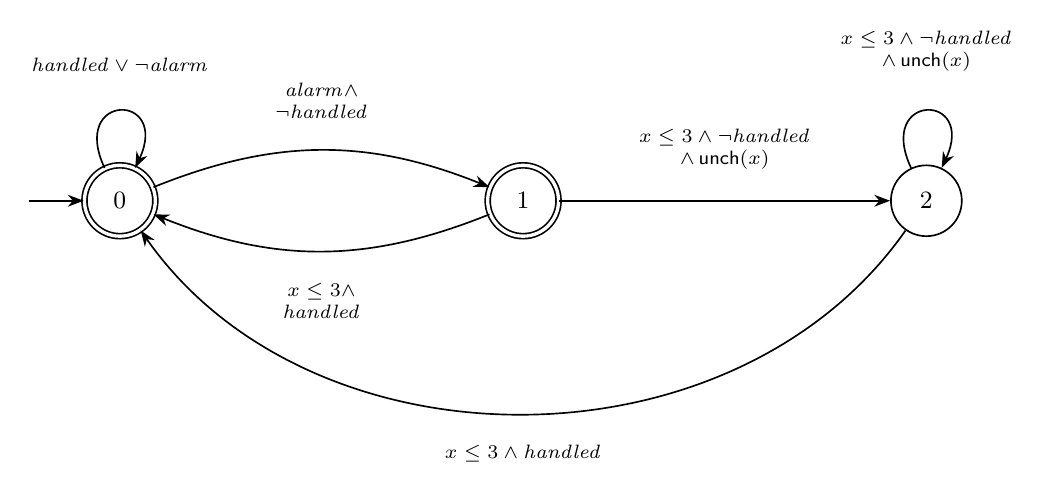
\begin{tikzpicture}[node distance=42mm]
  \node[fmaccept] (q0) {$0$};
  \node[fmaccept,right=of q0] (q1) {$1$};
  \node[fmstate,right=of q1] (q2) {$2$};
  \draw[fmedge] ([xshift=-7mm]q0.west) -- (q0.west);
  \draw[fmedge] (q0) edge[out=115,in=65,looseness=7] node[fmlabel,above=4.5mm]
    {$\mathit{handled}\lor\neg\mathit{alarm}$} (q0);
  \draw[fmedge] (q0) edge[bend left=22] node[fmlabel,above=3.5mm]
    {$\mathit{alarm}\land$\\$\neg\mathit{handled}$} (q1);
  \draw[fmedge] (q1) edge[bend left=22] node[fmlabel,below=3.5mm]
    {$x\le3\land$\\$\mathit{handled}$} (q0);
  \draw[fmedge] (q1) -- node[fmlabel,above=3.5mm]
    {$x\le3\land\neg\mathit{handled}$\\$\land\,\Unch(x)$} (q2);
  \draw[fmedge] (q2) edge[out=115,in=65,looseness=7] node[fmlabel,above=4.5mm]
    {$x\le3\land\neg\mathit{handled}$\\$\land\,\Unch(x)$} (q2);
  \draw[fmedge] (q2) edge[bend left=55] node[fmlabel,below=3.5mm]
    {$x\le3\land\mathit{handled}$} (q0);
\end{tikzpicture}
\caption{Propositional B\"uchi automaton redrawn from Spot's output for the
alarm-response formula. Edges are labeled by the full Boolean condition on
event and clock atoms. Double circles are accepting states, the incoming arrow
marks the initial state, $\Unch(x)$ is the preservation marker, and state
numbers are Spot's}
\Description{A three-state propositional Büchi automaton with edges labeled by Boolean conditions on the alarm and handled events and clock atoms; double circles mark accepting states and an incoming arrow marks the initial state.}
\label{fig:alarm-backend}
\end{figure*}
Rocq splits the disjunctive self-loop into two cubes. Lemma
\Rocqid{alarm_response_T_eq} matches its input to the Rocq translation;
\Rocqid{alarm_response_spot_backend_contract} proves that the transcribed
automaton has exactly that LTL language on the action-consistent propositional
words, which is the contract above. 
The resulting concrete TBA is \Rocqid{alarm_response_spot_tba}. It has initial
location $0$, accepting locations $\{0,1\}$, and clock $x$.
Figure~\ref{fig:alarm-tba} shows the reset-completed automaton of the Rocq
record. Each edge is labeled by its event, its clock guard, and its resets;
guards are checked before resets, and an edge without a guard is unconditional. The
two edges from $0$ to $0$ of the record are drawn as one edge with two labels.
\begin{figure*}[t]
\centering
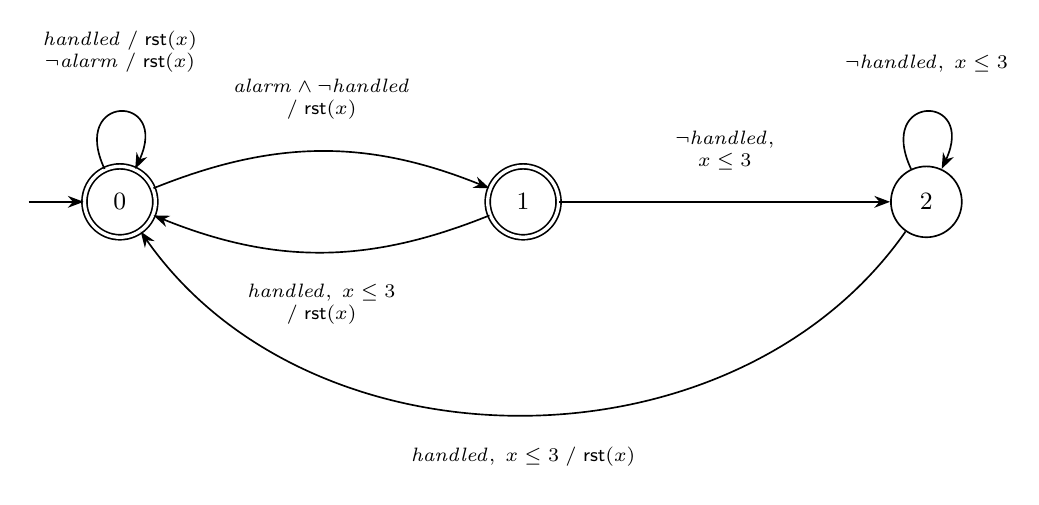
\begin{tikzpicture}[node distance=42mm]
  \node[fmaccept] (q0) {$0$};
  \node[fmaccept,right=of q0] (q1) {$1$};
  \node[fmstate,right=of q1] (q2) {$2$};
  \draw[fmedge] ([xshift=-7mm]q0.west) -- (q0.west);
  \draw[fmedge] (q0) edge[out=115,in=65,looseness=7] node[fmlabel,above=4.5mm]
    {$\mathit{handled}\;/\;\mathsf{rst}(x)$\\$\neg\mathit{alarm}\;/\;\mathsf{rst}(x)$} (q0);
  \draw[fmedge] (q0) edge[bend left=22] node[fmlabel,above=3.5mm]
    {$\mathit{alarm}\land\neg\mathit{handled}$\\$/\;\mathsf{rst}(x)$} (q1);
  \draw[fmedge] (q1) edge[bend left=22] node[fmlabel,below=3.5mm]
    {$\mathit{handled},\;x\le3$\\$/\;\mathsf{rst}(x)$} (q0);
  \draw[fmedge] (q1) -- node[fmlabel,above=3.5mm]
    {$\neg\mathit{handled},$\\$x\le3$} (q2);
  \draw[fmedge] (q2) edge[out=115,in=65,looseness=7] node[fmlabel,above=4.5mm]
    {$\neg\mathit{handled},\;x\le3$} (q2);
  \draw[fmedge] (q2) edge[bend left=55] node[fmlabel,below=3.5mm]
    {$\mathit{handled},\;x\le3\;/\;\mathsf{rst}(x)$} (q0);
\end{tikzpicture}
\caption{Timed automaton of the alarm-response Rocq record after relaxation
and reset completion. Edges are labeled by event, clock guard and, after a
slash, the clocks reset; double circles are accepting states. The Graphviz DOT
graph-to-record correspondence remains outside the Rocq proof}
\Description{A three-state timed automaton obtained from the propositional automaton by relaxation and reset completion; edges carry an event, a clock guard, and the clocks reset after a slash; double circles mark accepting states.}
\label{fig:alarm-tba}
\end{figure*}
The theorem \Rocqid{alarm_response_spot_tba_correct} instantiates
Theorem~\ref{thm:mtl-to-tba-correct} and proves that this record accepts
exactly the timed words satisfying $f_{\mathit{alarm}}$.


\section{Extracted Tool and Validation}
\label{sec:evaluation}
To exercise the verified definitions, we extract the functions $\T$,
relaxation, and reset completion to OCaml~\cite{letouzey_extraction} and wrap
them in a tool, \texttt{mtl2tba}. The verified claim of the article is Theorem~\ref{thm:mtl-to-tba-correct}; the
tool is not needed for it.

\subsection{Tool and trust boundary}
\label{subsec:workflow}
\texttt{mtl2tba} parses an MTL formula, computes $\T(f)$, calls
Spot~2.16~\cite{spot} as the LTL-to-B\"uchi backend, reads its LBTT output, and
applies relaxation and reset completion. We write
$\mathsf{compile}(f)=\mathsf{compile\_with}(A)$, where $A$ is the automaton that
Spot returns for $\T(f)$. The functions $\T$, relaxation, and reset completion
are extracted from the Rocq definitions, so the executable functions correspond to the Rocq definitions that
Theorem~\ref{thm:mtl-to-tba-correct} covers, relative to the backend contract
and assuming that extraction and the OCaml toolchain are correct. Bounds are
integers in the tool, whereas the theorem is stated for real bounds. The verified backend of Section~\ref{subsec:verified-backend} is not
part of the tool. Outside the checked boundary are the parser and the printers, the call
to Spot and the LBTT import (covered only by Assumption~\ref{ass:backend}), and the extraction to OCaml and the OCaml compiler. Spot returns
automata with transition-based, possibly generalized acceptance; their
conversion to the propositional automaton of Assumption~\ref{ass:backend} is
part of this unverified import, and the tool does not check at run time that
Spot's output meets the contract. The compiled TBAs are exported to TChecker in
a textual format; that the exported automaton has the semantics of the Rocq
TBA (guards tested before resets at each event, no invariants, one event per
position) is likewise unverified.

The artifact (\path{evaluation/} and \path{case_study/}) contains the scripts
that run the tool on sample formulas and a two-train railway-crossing model with
TChecker. The article makes no claim based on their results.


\section{Artifact}
\label{sec:artifact}
The Rocq sources, the assumptions report, the tool \texttt{mtl2tba}, the
evaluation scripts with their inputs and raw results, the case study, and the
Spot input and graph of the alarm-response example are archived on Zenodo
(\url{https://doi.org/10.5281/zenodo.23916521}~\cite{fares_zenodo_artifact}) and
developed at \url{https://github.com/efares1/rocq-mtl-to-tba-translation}; the
revision described here is the release tagged \texttt{v1.15}. The development has about 10,000 lines of Rocq in thirteen files
(the core definitions, the encoding correctness proof, the alarm instance, the
zero-initialization corollary, the assumptions check, five files for the
verified backend, and three files for the compilation theorem for
polarity-correct clocked LTL, its MTL instance and the non-MTL examples) and
builds with
Rocq~9.0.1 (\texttt{make} in \path{proof/}); \path{proof/CheckAssumptions.v}
prints the assumptions of the main theorems, which are recorded in
\path{proof/ASSUMPTIONS.txt}, and \texttt{coqchk} re-checks the compiled
objects. The main claims have direct source declarations:
\Rocqid{EncodingCorrect_proved} and \Rocqid{canonical_encoding_all} establish
the formula-to-clocked-LTL equivalence, \Rocqid{MTL_to_TBA_correct_with}
composes it with the backend contract,
\Rocqid{MTL_to_TBA_correct_verified} with the verified backend, and
\Rocqid{alarm_response_spot_tba_correct} is the concrete alarm instance
(Section~\ref{sec:alarm-example}). Two Python scripts audit the alarm
instance and the finite overlap scenarios of
Table~\ref{tab:overlap-example}; they are executable audits, not verified
components. The scripts in \path{evaluation/} and \path{case_study/} run the tool, under
Linux or WSL with OCaml, Spot~2.16, TChecker~0.8, and ltl2ba~1.3; no claim of the
article depends on their results.

\section{Related Work}
\label{sec:related}

Pointwise MTL has extensive decidability and expressiveness results
\cite{RK90,RTH96,MTLsem,ouaknine_worrell_lics05,
bouyer_chevalier_markey_fsttcs05}. Unrestricted dense-time MTL has no general
effective translation to finite ordinary timed automata; bounded-variability
and alternating-automaton results have different scopes
\cite{nickovic_piterman_formats10,BM14}. MTL$_{0,\infty}$ retains common
response and separation properties~\cite{RTH96,BDLG14}. The hatted
operators make the timing reference explicit in the logic and proof.

\runinhead{Translations of timed logics.}
Li et~al. prove the full-fragment language-equivalence result in an appendix
of the version we consulted, again omitting the remaining cases as similar.
Bulychev et~al. prove theirs for the safety and co-safety
fragments, with several cases omitted as similar to the cases shown. As we read
them, the rewriting rules of both cover only the non-strict ordinary operators and assume that no other timed
operator occurs; strict bounds and the hatted operators appear in their
semantics but not in their rules.
The Rocq development covers all eight primitive cases and derives the ordinary
operators from them. Our overlapping-activation proof checks completeness for the present
formal model; we do not infer that prior constructions lacked such handling.
The reset rule of our completion, in which a preservation clock is reset unless
the cube requires $\Unch$ and a restart clock is reset only when the cube
requires $\Reset$, corresponds, as we read them, to the best-choice policy of Bulychev et~al.
and Li et~al.; the language equality we prove is for the automaton built with
it.

Bulychev et~al. state that their translation uses ``the classical
tableau-based translation from linear-time temporal formulas into B\"uchi
automata'' with two modifications: no B\"uchi acceptance condition for the
safety and co-safety fragments, and an auxiliary clock for each timed
subformula. Li et~al. proceed by a closure, extended formulas that carry the
clock bookkeeping, a normal form, a transition-based timed B\"uchi automaton,
and a degeneralization step. In both, as we read them, the timed expansion and the B\"uchi
construction are one hand-built construction. Ours differs in architecture:
the formula is encoded into untimed clocked LTL, any LTL-to-B\"uchi backend
may then be used, and its correctness enters the composed theorem as an
explicit contract. This factoring is what the Rocq development exploits, and
it is also why the backend contract is separate from the timed argument.
To the best of our knowledge, none of the translations from MTL or MITL to
timed automata that we examined (the two above, the testers of Maler et~al.,
MightyL, MightyPPL, and Xu and Miao) is presented in this form; we examined
the cited works to different depths. The tester-based constructions of Maler
et~al. also separate timed observers from an untimed core; we have not compared
the two architectures in detail, and the claim is limited accordingly.

Xu and Miao describe a PVS-based transformation from MITL formulas to fair
timed automata, including construction principles and implementation
details~\cite{xu08}. Their construction builds one tester automaton per
subformula, each with local clocks that measure the elapsed time against the
metric interval, and composes the testers in parallel; it has no intermediate
untimed LTL stage. As far as we can tell from the cited paper, PVS is used to implement the
transformation; we have not established whether a correctness proof was
mechanized. This is an earlier proof-assistant-based timed-logic translation;
our scope-specific comparison concerns the pointwise
MTL$_{0,\infty}$ construction formalized here.

MITL translations use temporal testers, automata networks, or one-clock
alternating automata~\cite{maler_mitl_to_ta,
ferrere2019_realtimelogic_to_ta,BM14}; MightyL and MITL2Timed provide
UPPAAL-oriented tools for that distinct logic
\cite{mightyl_paper17,mitl2timed_github}. MightyL, for example, outputs a
network of timed automata, one per temporal subformula, generalizing the
Gastin--Oddoux LTL-to-B\"uchi construction~\cite{ltl2ba_cav01}; as described in~\cite{mightyl_paper17}, it does not call an LTL-to-B\"uchi
tool on a timed formula. Obligation-merging techniques are
related, while our one-sided residual predicates support the checked
completeness proof.

\runinhead{Clocked temporal logic and subformula clocks.}
The clocked linear temporal logic extension CLTLoc adds clock comparisons and reset predicates and has been used to
encode metric logics~\cite{bersani_cltloc}. Our propositional vocabulary
is similar, but it serves as an intermediate language for automaton synthesis: the backend treats clock
tests and reset markers as propositions. Positivity gives upward closure, and
reset completion restores timed meaning; hence the explicit relaxation proof.

Event-clock logics associate clocks with subformulas to measure time since or
until events~\cite{afh_eventclock_tcs99,
raskin_schobbens_jalc99,nickovic_piterman_formats10}. Formula-indexed clocks
are established; what we add is a machine-checked proof that one clock per
distinct timed formula preserves language across repeated activations and all
cases (Section~\ref{subsec:occurrence-induction}).

\runinhead{Recent automata-based real-time verification.}
Recent neighboring work addresses different settings: an improved one-clock
alternating MTL automaton for finite timed words with clock deactivation and
zone analysis~\cite{bouyer_srivathsan_vishwanath_fossacs25}; and TEMPORA's
pointwise MITL model checking with past and future modalities~\cite{akshay_et_al_tempora26}. These do not
translate our MTL$_{0,\infty}$ fragment to infinite-word TBAs.
Ho et~al.'s MightyPPL translates pointwise MITL with past and Pnueli
modalities over finite and infinite timed words; it gives mathematical
construction results and proof sketches alongside a complete implementation
whose testers sequentialize overlapping obligations~\cite{mightyppl_tacas26}. A companion
preprint~\cite{mightyppl_qest_arxiv26} describes
an implementation for existentially punctual metric temporal logic with past
and Pnueli modalities (MTLPPL). In that preprint, the term
\emph{one-sided MTL} denotes the subfragment without past or Pnueli modalities, whereas
here it describes interval shapes $[0,d]$ and $[d,\infty)$. Any syntactic
containment comparison is limited to conventional source formulas after
zero-bound reduction and with integer bounds; it excludes hatted abstract syntax tree
constructors. The fragment of that preprint also permits punctual and non-one-sided
intervals in its stated positions; differing bounds and timed-word
conventions preclude a shared-input semantic comparison.

These tools (TEMPORA, MightyPPL, and the alternating-automaton work above)
address different fragments or output models; we neither re-verify
them nor make a shared-input, coverage, clock-count, or performance
comparison with them. The Rocq development is not integrated with CASAAL,
MightyPPL, or another checker.

\runinhead{Mechanized translations and trusted backends.}
Proof-assistant work already verifies LTL-to-B\"uchi constructions and model
checkers~\cite{schimpf_tphols09,cava_cav13,ltl_to_gba_afp,
seidl_sickert_afp19}. Jantsch and Norrish verify in HOL4 a translation of LTL to
generalized B\"uchi automata via very weak alternating automata, and obtain
verified machine code for it with CakeML~\cite{jantsch_norrish_itp18}. Our construction is
simpler and less efficient; its purpose is to discharge the backend contract in
Rocq, the system of the translation proof. Wang et~al. verify an MLTL-to-regular-expression
transformation in Isabelle/HOL, export executable code, and compare it with
existing implementations~\cite{wang_mltl_tacas25}. Chattopadhyay and
Mamouras formalize in Coq a compositional construction of online monitors for
past-time MTL over a discrete temporal domain, using quantitative semantics
and Moore machines; they also extract OCaml monitors. This is a distinct
monitoring target and semantic setting from the infinite-word TBA construction
studied here~\cite{chattopadhyay_mamouras_rv20}. For metric logics, Roohi
and Viswanathan use PVS to correct an unsound release semantics in prior MITL
decision procedures and prove supporting results for an adapted
timed-automata construction under continuous-time signal semantics~\cite{roohi_viswanathan_vmcai18}. Xu and Miao's PVS-based construction is
described above. On the downstream side, Wimmer and Lammich verify in
Isabelle/HOL a model checker for reachability in timed automata, with the tool
Munta, and Wimmer and von Mutius verify a certificate checker for reachability~\cite{munta_tacas18,munta_formats19,wimmer_vonmutius_tacas20}; as we read
them, these cover reachability and not B\"uchi emptiness or the translation of a
timed logic, so they complement the unverified TChecker step in a model-checking flow. Basin et~al. verify in Isabelle/HOL an optimized
monitor for metric first-order dynamic logic~\cite{basin_verimon_ijcar20}, again
a monitoring target. These works are proof-assistant
precedents for related metric logics, monitors, and automata; the present
development is a Rocq-checked correctness proof for the specified pointwise
infinite-word TBA construction. In web searches we found no proof-assistant
formalization of a translation from MTL or MITL to timed automata other than
the PVS work above; this does not exclude unpublished or unindexed
developments.

\runinhead{Event-B refinement patterns.}
This article is part of a line of research on generating Event-B refinement
patterns from timed requirements: the TBA produced by the translation is the
input of the pattern-generation step. Our earlier work on Event-B patterns
covers their DSL-based generation~\cite{fares_abz23}, their derivation through
weakest preconditions~\cite{fares_facs24}, and predicate
transformers~\cite{fares_scp27}. The present paper provides the verified
MTL-to-TBA stage and illustrates, in Section~\ref{sec:evaluation}, that the same
automata can be composed with timed system models for model checking.


\section{Conclusion}
\label{sec:conclusion}
We have given a Rocq-checked soundness-and-completeness development for the
pointwise MTL$_{0,\infty}$-to-TBA construction, factored through an untimed
clocked-LTL formula and a standard LTL-to-B\"uchi backend. The proof covers all
eight primitive cases, soundness for arbitrary clock-consistent reset traces,
and completeness using one canonical trace across repeated activations of
formula-keyed clocks; the occurrence-indexed induction connects each syntactic
occurrence to its translation while preserving the identity of a shared clock.
Relaxation and reset completion are checked and composed with a propositional
backend through an explicit language-equivalence contract, which we discharge
for a verified LTL-to-B\"uchi construction. The work builds on the
language-equality results of Bulychev et~al. and Li et~al. and on adjacent
proof-assistant work, and adds the factored reformulation with a
machine-checked proof for the semantic model defined
here~\cite{li_spin7,xu08,roohi_viswanathan_vmcai18}. A second main result isolates
relaxation and reset completion from MTL: they are proved for every
polarity-correct positive clocked-LTL formula over an abstract clock type, with the MTL translation as a checked
instance and counterexamples showing that the polarity condition cannot be
omitted for this reset rule; whether other
timed logics can be compiled through the same stage by proving only an encoding
equivalence is left open.

The theorem applies to the stated pointwise semantics. With the verified
backend it holds unconditionally; for the Spot-based tool it is
relative to the contract. The contract is proved for a manual
transcription of Spot's output on one formula (the alarm-response record, whose
fidelity to Spot is checked by inspection only). Spot's graph generation,
the graph import, the parser, and the extraction lie outside the checked
boundary.
Future work includes verifying an efficient LTL-to-B\"uchi translation or checking Spot's output
against the contract, extending the mechanization to the surrounding tool, and
optimizing the generated automata and comparing them with other translators.

\begin{acks}
This research did not receive any specific grant from funding agencies in the
public, commercial, or not-for-profit sectors. During the preparation of this
work the authors used Claude (Anthropic) to improve the manuscript text, to
generate evaluation and checking scripts, and to assist the
development of parts of the Rocq sources, namely in the Rocq formalization of the verified LTL-to-B\"uchi backend. After using this tool, we have reviewed and
edited the content as needed and take full responsibility for the content of the
article. All theorems whose Rocq declaration is named were checked with Rocq;
the prose arguments in the text summarize those proofs, and the Rocq sources
are authoritative.
\end{acks}

\textbf{Data availability.} The Rocq development, the \texttt{mtl2tba} tool, the evaluation scripts with their inputs and raw results, and the examples are archived on Zenodo with the persistent identifier \url{https://doi.org/10.5281/zenodo.23916521}~\cite{fares_zenodo_artifact}, and developed at \url{https://github.com/efares1/rocq-mtl-to-tba-translation}.

\bibliographystyle{ACM-Reference-Format}
\bibliography{references}

\end{document}
